
\renewcommand\chapterillustration{abertura-medidas}
\renewcommand\chapterwhat{As noções presentes no ato de medir, a necessidade de padronização das unidades de medida e o sistema internacional de medidas. Medidas da informática e a medida da informação. Unidades de medida que são compostas por outras unidades de medida e algumas de suas aplicações. Um breve panorama histórico da evolução da precisão em algumas medidas e suas consequências. Normas para alguns tipos de valores obtidos nas medições: Notação científica, ordem de grandeza e algarismos significativos; aproximações e medidas representadas por números irracionais.}

\renewcommand\chapterbecause{Planejamento de consumo familiar, cumprimento de horários, comparação e aquisição de bens de consumo, são apenas algumas das situações do cotidiano de uma pessoa comum. Em todas elas unidades de medida, estimativas ou medições precisam ser conhecidas, manipuladas ou obtidas. 

A evolução científico-social humana já se incumbiu de criar unidades de medidas: tempo, força, temperatura, luz e etc. A pesquisa e a criatividade demonstram que a geração de novas tecnologias ou novos olhares sobre os processos tendem a necessitar de novas unidades. Um cidadão integral precisa ter autonomia para entender o que está por vir.  É nesse contexto que se desenvolveu esse estudo. Para que possam aprender a ler, entender e usar na sua comunicação as unidades de medidas, da estimativa à precisão, tal qual a utilizamos no ato de medir.}
\chapter{Unidades de medidas e ordem de grandeza}

\mbox{}\thispagestyle{empty}\clearpage
0
\thispagestyle{empty}

\begin{center}
Projeto: LIVRO ABERTO DE MATEMÁTICA

\noindent \begin{tabular}{lcccr}

\includegraphics[scale=.15]{impa}& \quad\quad& 
\includegraphics[width=3cm]{logo} & \quad\quad& 
\includegraphics[scale=.24]{obmep} 
\end{tabular}
\end{center}

\vspace*{.3cm}

Cadastre-se como colaborador no site do projeto: \url{umlivroaberto.org}

Versão digital do capítulo:

\url{https://www.umlivroaberto.org/BookCloud/Volume_1/master/view/PE104.html}

% \begin{center}
%   \includegraphics[width=2cm]{canvas}
% \end{center}

\begin{tabular}{p{.15\textwidth}p{.7\textwidth}}
Título: & Unidades de Medida e Ordens de Grandeza\\
Ano/ Versão: & 2020 / versão 1.0 de \today\\
\\
Editora & Instituto Nacional de Matem\'atica Pura e Aplicada (IMPA-OS)\\
\\
Realização:& Olimp\'iada Brasileira de Matem\'atica das Escolas P\'ublicas (OBMEP)\\
\\
Produção:& Associação Livro Aberto\\
\\
Coordenação: & Fabio Simas e Augusto Teixeira (livroaberto@impa.br)\\
\\
Autores: & Bruno Viana (Colégio Pedro II), \\
 		 & Luiz Amorim Duarte, \\
 		 & Maria de Fátima,\\
\\
Revisão: & Wanderley Rezende \\
\\
Design: & Andreza Moreira (Tangentes Design) \\
\\
Ilustrações: & Luiz Amorim Duarte \\ 
\\
Gráficos: & Tarso Caldas (Licenciando da UNIRIO) \\
\\
Capa: & Foto de Taneli Lahtinen, no Unsplash \\
	  & https://unsplash.com/photos/g\_LKoKQNr44 \\

\end{tabular}
\vspace{.5cm}


\begin{figure}[b]
\begin{minipage}[l]{5cm}
\centering

{\large Licença:}

  
\includegraphics[width=3.5cm]{cc-by-sa1}
\end{minipage}\hfill
\begin{minipage}[c]{5cm}
\centering
{\large Desenvolvido por}


\includegraphics[width=2.5cm]{logo-associacao.jpg}
\end{minipage}
\begin{minipage}[r]{5cm}
\centering

{\large Patrocínio:}
  \vspace{1em}
  
\includegraphics[width=3.5cm]{itau}
\end{minipage}
\end{figure}

\mainmatter

\label{\detokenize{NO103::doc}}\label{\detokenize{NO103:unidades-de-medidas-e-ordem-de-grandeza}}

\explore{Qual é a medida?}
\label{\detokenize{NO103-0:explorando-qual-e-a-medida}}\label{\detokenize{NO103-0::doc}}


A análise da história do ser humano, seus hábitos e os desenvolvimentos sociais e tecnológicos revelam em vários momentos uma necessidade em estabelecer uma referência para contar objetos e medir. Cada um de nós, desenvolvendo nossas faculdades, num ambiente que já tem diversos desses referenciais estabelecidos, vemos com muita naturalidade muitos desses referenciais de contagem.

Quando bebês, nos vemos obrigados, pouco a pouco, a aprender a dormir mais no horário em que, a céu aberto, está mais escuro. Temos a necessidade de certa quantidade de alimento em períodos específicos. Vemos nossos responsáveis nos pesando e nos medindo e reagindo com alegria ou tristeza de acordo com a análise especializada desses dados. Ou seja, na atualidade, nossa entrada na vida já vem carregada de contagens e medidas.

Neste capítulo vamos trazer um pouco de reflexão sobre algumas dessas medidas, possibilitando o entendimento da busca humana em desenvolver, utilizar e até adequar essas referências que compõe hoje o ato de medir.
\phantomsection\label{\detokenize{NO103-0:ativ-unidades-de-medidas-uma-recomendacao-medica}}
\begin{task}{Uma recomendação médica}

Após uma consulta médica, uma pessoa é orientada a manter alguma atividade física regular. A médica foi específica: - “Caminhe três quilômetros por dia, com tênis adequado, roupas leves e se hidratando”!


\begin{figure}[H]
\centering
\capstart
\begin{multicols}{2}
\noindent\includegraphics[width=200bp, trim={0 0 9.1cm 0}, clip]{{LA_UM_Ativ1_1}.png}

\begin{tikzpicture}[scale=2.35, every node/.style={scale=1.5}]

\draw [fill=secundario!50] (-1.5,-1) rectangle (1.5,1);

\draw [fill=white] (-1.3,-.8) rectangle (1.3,.8);

\node [align=center] {Representação \\ do caminho \\ visto de cima};
\end{tikzpicture}
\end{multicols}
\caption{Imagem ao lado da foto elaborada por Luiz Amorim Duarte}\label{\detokenize{NO103-0:fig-ativ-recomendacao-medica-praca}}\label{\detokenize{NO103-0:id1}}\end{figure}



Essa pessoa se prepara e vai até a praça. Chegando lá depara-se com um problema. Como saber quantas voltas são necessárias na pista da praça para cumprir a recomendação médica? Como essa pessoa, sem nenhum instrumento de medida, poderá seguir a indicação médica?…

Para responder a essas perguntas, vamos precisar de um planejamento.
\begin{enumerate}
\item {} 
Reflita um pouco na situação e indique, quais as medidas que a pessoa precisa conhecer para iniciar as recomendações médicas?

\item {} 
Tente sugerir três objetos cuja medida seja fácil de obter e que dariam conta do problema. Converse sobre a escolha desses objetos com os outros estudantes.

\item {} 
Como a pessoa deve utilizar cada um desses objetos de medida conhecida para resolver o problema?

\item {} 
Como a situação envolve conhecer distância percorrida a pé, qual dessas medidas parecem mais adequadas para a resolução do problema:

$\Box$ o pé da pessoa.

$\Box$ a altura da pessoa.

$\Box$ o passo da pessoa.

\item {} 
Descreva como, com a escolha feita no item anterior, a pessoa deve proceder para obter a medida que precisa. Compare sua descrição com a de outros estudantes.

\item {} 
O que você considera mais adequado: Utilizar a medida escolhida (tamanho do pé, altura ou tamanho do passo) do início ao fim da caminhada, ou seja, até completar os três quilômetros; ou é melhor usar essa medida para obter o comprimento de uma volta na pista e, com isso, contar os três quilômetros?

\item {} 
Converse com outros estudantes e cite o que poderia ser medido na sua escola, utilizando a mesma técnica dos três quilômetros de caminhada; escolham, juntos, uma das que foram citadas e realizem essa medição.

\item {} 
Por mais quatro vezes, meça o que mediu no item anterior, utilizando a mesma técnica. Essas medidas são todas iguais? Foram iguais para os outros estudantes? Por quê?

\item {} 
É provável que você ou os outros estudantes tenham obtido medidas diferentes dentre as cinco medições feitas. Como tratar esses valores com a finalidade de informar para alguém a melhor estimativa para o comprimento investigado?

\item {} 
Para melhor adequar essa atividade ao seu tempo disponível, como a pessoa deveria proceder para obter a estimativa de tempo que levará para percorrer os três quilômetros?

\end{enumerate}
\end{task}


\begin{task}{A lotação no restaurante}
\label{ativ-nome-do-capitulo-nome-da-atividade}



Um empresário encontrou um lugar que parecia estar adequado aos seus planos de montar um restaurante. Com a finalidade de tomar sua decisão sobre a aquisição ou não deste lugar, precisava de mais detalhes que só uma visita poderia fornecer. Pediu ao seu irmão mais novo que visitasse o lugar e lhe trouxesse informações de que precisava. Enviando seu irmão mais novo, ao invés de uma pessoa especializada, o empresário tem a intenção de ajudar seu irmão a adquirir experiência em empreendedorismo.

O irmão mais novo retornou da visita com a figura a seguir e afirmou:  - “Esta é a vista de cima da região destinada às mesas para os clientes. O  “quadriculado”  é o piso desta região”.

\begin{figure}[H]
\centering

\includegraphics[width=430bp]{{LA_UM_Ativ2}.png}
\caption{Imagem produzida por Luiz Amorim Duarte}
\label{\detokenize{NO103-0:fig-unidades-de-medidas-ativ-a-lotacao-no-reataurante}}
\label{\detokenize{NO103-0:id2}}
\end{figure}

E continuou: - “Também fiz um esboço dos conjuntos mesa-cadeiras que serão utilizados no restaurante”.

\begin{figure}[H]
\centering


\noindent
\includegraphics[width=400bp]{{LA_UM_Ativ2-2}.png}
\caption{Imagem produzida por Luiz Amorim Duarte}
\label{\detokenize{NO103-0:fig-unidades-de-medidas-ativ-a-lotacao-no-restaurante2}}
\label{\detokenize{NO103-0:id3}}
\end{figure}

Considerando as informações trazidas pelo irmão mais novo, tente fazer o que se pede a seguir.
\begin{enumerate}
\item {} 
Coloque uma folha fina de papel sobre os esboços dos conjuntos mesa-cadeiras, cubra com um lápis os desenhos várias vezes e recorte-os de modo a ficar um conjunto mesa-cadeira em cada pedaço. Feito isso, tente posicioná-los no desenho do salão para estimar qual seria a quantidade máxima de clientes (lotação) possível para este salão.

\item {} 
De acordo com sua análise da lotação e considerando que cada lugar gere um lucro de R\$ 10,00 por hora, qual o lucro esperado para uma hora de funcionamento com a lotação completa?

\item {} 
Os outros estudantes concordam com sua resposta do item anterior? Por quê?

\item {} 
Seria suficiente, ou mesmo adequado, fazer uma média das lotações obtidas por todos os estudantes e tomar essa média como sendo a real lotação do salão?

\item {} 
Que informações você identifica que poderiam ter sido trazidas pelo irmão mais novo, afim de melhorar a estimativa da lotação?

\end{enumerate}
\end{task}



A base do comércio é a troca. Alguém oferece a posse de certo objeto e avisa as condições que considera justas para que você possa adquirir o tal objeto. Essas condições, podem envolver dinheiro, outros objetos, serviços, etc. Caso você considere justo, a comercialização do objeto acontece, ou seja, a troca é efetivada!

Nesta atividade, vamos nos colocar numa destas situações comerciais. As informações aqui presentes estão simplificadas para o objetivo da atividade, todos os detalhes podem ser obtidos em:

Cultura de Maçã: “\url{http://www.sebrae.com.br/sites/PortalSebrae/artigos/o-cultivo-e-o-mercado-da-maca,ea7a9e665b182410VgnVCM100000b272010aRCRD}” e “\url{https://ainfo.cnptia.embrapa.br/digital/bitstream/item/162029/1/A-cultura-da-maca.pdf}”

Cultura de Banana: “\url{http://www.ufrgs.br/alimentus1/feira/mpfruta/banana/industi.htm}” e “\url{http://www.scielo.br/pdf/rbf/v31n3/a18v31n3.pdf}”
\begin{task}{comparando maçãs com bananas}
\label{ativ-unidades-de-medida-macas-e-bananas}

Os vizinhos Antônio e Fernando cultivam a terra como um meio de sustento. Antônio, dentre outras coisas, cultiva maçãs; Fernando cultiva algumas bananeiras. Uma das macieiras de Antônio produz uma média de 180 frutos por ano, sempre em torno dos meses de janeiro, fevereiro e março; Já uma bananeira de Fernando produz, em média, 2 cachos por mês, totalizando 20 pencas, cada penca com 15 bananas.

\begin{figure}[H]
\centering
\capstart

\noindent\includegraphics[width=350bp]{{LA_UM_Ativ3}.png}
\caption{Imagem adaptada por Luiz Amorim Duarte}\label{\detokenize{NO103-0:fig-unidades-de-medidas-ativ3}}\label{\detokenize{NO103-0:id4}}\end{figure}
\begin{enumerate}
\item {} 
Em média, quantas bananas Fernando obtém em cada bananeira em um mês?

\item {} 
Distribuindo toda a produção de uma macieira de Antônio para cada mês do ano, quantas maçãs ele teria em um mês?

\item {} 
Agora que já foi calculado quantas frutas, Fernando e Antônio, tem disponíveis, em um mês e considerando a produção de apenas uma de suas árvores, eles vão estabelecer uma relação de troca. Usando apenas essas quantidades mensais de frutas como critério de troca, uma maçã deve ser trocada por quantas bananas?


\begin{center}

\begin{tabulary}{\linewidth}[t]{|T|}
\hline

\textbf{Geléia de Maçã}

A família de Antônio não consome todas as maçãs que produz por estação, sendo assim, antes que a produção apodreça, ele faz geleia com as maçãs e as embala em potes. Considere que 100 maçãs sejam usadas para a receita da geleia, que depois de pronta, rende 40 potes com validade de um ano.
\\
\hline
\end{tabulary}
\end{center}

\item {} 
Considerando só bananas e maçãs produzidas por ano e de uma única árvore de cada espécie, estabeleça quantas bananas seriam dadas em troca de um pote de geleia de maçã?

\item {} 
Para fazer a geleia de maçã, além das maçãs, gastam-se outros ingredientes, o trabalho dedicado ao tempo do preparo, os potes, etc. Pensando nisso, Antônio resolveu adicionar para cada pote de geleia um custo, em maçãs, de mais 75\%. Quanto fica agora o valor de um pote de geléia, em bananas?

\item {} 
O resultado do valor de um pote de geleia, em bananas, calculado no item anterior, exigiria meia banana na troca. Sugira uma troca em que essa meia banana não apareça.

\item {} 
Você considera prático e justo o sistema de troca adotado nesta atividade? E se Antônio e Fernando tivessem outros produtos: café, gado leiteiro, algodão, galinhas… o estilo de troca é eficiente? O que parece faltar nessa dinâmica?

\end{enumerate}
\end{task}

\arrange{Um pouco de história}
\label{\detokenize{NO103-0:organizando-as-ideias-um-pouco-de-historia}}
Em nossas vidas estamos cercados por informações numéricas que, geralmente, possuem uma certa natureza, ou seja, estão acompanhadas de uma descrição. As atividades nos revelam que, o estabelecimento de um padrão, representa a única opção quando existe a necessidade de estimar, fazer o registro dessa estimativa ou comunicá-la para outras pessoas, seja para informar, planejar ou negociar.

Ao longo da história, diversas unidades foram criadas em diversos lugares, inicialmente tendo como referência alguma parte do corpo ou objeto físico. O livro “A Informação”, de James Gleick, conta que o primeiro registro oficial feito por um país ocorreu no século XII por Ricardo I, que reinou de 1189 a 1199 na Inglaterra. Ele determinou unidades para as grandezas simples: comprimento e  capacidade. Acredita-se que a grande motivação para o estabelecimento oficial destas unidades tenha sido o comércio. Sem uma padronização no comércio, é fácil imaginar que dois conhecidos paguem preços iguais para quantidades diferentes, fazendo um deles ficar com a sensação de que foi enganado. Não é difícil perceber que, mantendo as coisas dessa forma, haveria um grande problema em se manter a ordem e a paz nesse lugar. Resta assim, uma única saída: estabelecer padrões e regras que evitem essas situações desagradáveis.

Em 1790, a França reúne diversos cientista e cria um sistema métrico, de onde surge o metro, que vem do grego \emph{métron} e significa “o que mede”. Na época, o metro ficou estabelecido como $\displaystyle\frac{1}{10.000.000} = 10^{-7}$ da distância entre o Pólo Norte e o Equador.

\begin{figure}[H]
\centering
\capstart

\noindent\includegraphics[width=150bp]{{LA_Metro}.png}
\caption{O metro era a distância do Pólo Norte à linha do Equador dividida por dez milhões.}\label{\detokenize{NO103-0:id5}}\end{figure}

Com o tempo, os cientistas perceberam o quanto avanços de tecnologia e métodos poderiam “atualizar” os valores padronizados. Surge então a necessidade de reavaliar de tempo em tempo essas unidades. É assim que são formadas as Conferências Gerais de Pesos e Medida, que em 1983 aperfeiçoa o metro para o comprimento do trajeto percorrido pela luz no vácuo durante um intervalo de tempo igual a $\displaystyle\frac{1}{299.792.458}$ de um segundo. É claro que essa referência para o metro já demonstra o quanto de tecnologia foi necessária a esta padronização, que seria inimaginável num Egito que utilizava o \textbf{cúbito} (distância do cotovelo ao dedo médio do faraó) como unidade de medida de comprimento.

Na XI Conferência Internacional de Pesos e Medidas, realizada em 1960, adota-se o SI (Sistema Internacional de Unidades), responsável por apresentar as unidades padrão ou unidades simples. As imagens a seguir mostram um pouco do que foi estabelecido nesta conferência:



\begin{quote}
\begin{description}
\item[2.1.1.1 Unidade de comprimento (metro)] A definição do metro, dada em 1889, baseada no protótipo internacional de liga metálica de platina-irídio, foi substituída na 11$^{\text{a}}$ CGPM (1960) por outra definição baseada no comprimento de onda de uma radiação do criptônio 86. Esta mudança teve a finalidade de aumentar a exatidão da realização da definição do metro, realização esta conseguida com um interferômetro e um microscópio deslizante para medir a diferença do caminho óptico à medida que as franjas eram contadas. Por sua vez, esta definição foi substituída em 1983 pela 17$^{\text{a}}$ CGPM (1983, Resolução 1; CR 97 e Metrologia, 1984, 20, 25) pela definição atual seguinte:

\begin{quote}\textbf{O metro é o comprimento do trajeto percorrido pela luz no vácuo durante um intervalo de tempo de 1/299.792.458 de segundo.}\end{quote}

Essa definição tem o efeito de fixar a velocidade da luz no vácuo em 299.792.458 m/s.

O protótipo internacional original do metro, que foi sancionado pela 1$^{\text{a}}$ CGPM em 1889 (CR, 34-38), ainda é conservado no BIPM nas mesmas condições que foram especificadas em 1889.

\flushright (Página 24 da 1ª Edição Brasileira do Sistema Internacional de Unidades, disponível em \href{http://www.inmetro.gov.br/inovacao/publicacoes/si\_versao\_final.pdf}{SI INMETRO})
\end{description}
\end{quote}

\textbf{Definição dos símbolos para algumas das unidades}

\begin{table}[H]
\centering
\begin{tabu} to \textwidth{|l|l|l|l|}
\hline
\multicolumn{2}{|c|}{\cellcolor{\currentcolor!80}\textcolor{black}{\textbf{Grandeza de base}}} & \multicolumn{2}{c|}{\cellcolor{\currentcolor!80}\textcolor{black}{\textbf{Unidade de base do SI}}} \\
\hline
Nome & Símbolo & Nome & Símbolo \\
\hline
comprimento & $l,x,r,$ etc. & metro & m \\
\hline
massa & $m$ & kilograma & kg \\
\hline
tempo, duração & $t$ & segundo & s \\
\hline
\end{tabu}
\caption{Unidades de Base do SI, página 28 da 1$^{\text{a}}$ Edição Brasileira do SI}
\end{table}

\textbf{Definição de nomenclatura para múltiplos e fracionamentos das unidades}

\begin{table}[H]
\centering
\setlength\tabulinesep{1mm}
\begin{tabu} to \textwidth{|c|c|c|c|c|c|}
\hline
\thead
Fator & Nome do Prefixo & Símbolo & Fator & Nome do Prefixo & Símbolo \\
\hline
$10^1$ & deca & da & $10^{-1}$ & deci & d \\
\hline
$10^2$ & hecto & h & $10^{-2}$ & centi & c \\
\hline
$10^3$ & kilo & k & $10^{-3}$ & mili & m \\ 
\hline
$10^6$ & mega & M & $10^{-6}$ & micro & $\mu$ \\
\hline
$10^9$ & giga & G & $10^{-9}$ & nano & n \\
\hline
$10^{12}$ & tera & T & $10^{-12}$ & pico & p \\ 
\hline
$10^{15}$ & peta & P & $10^{-15}$ & femto & f \\
\hline
$10^{18}$ & exa & E & $10^{-18}$ & atto & a \\
\hline
$10^{21}$ & zetta & Z & $10^{-21}$ & zepto & z \\
\hline
$10^{24}$ & yotta & Y & $10^{-24}$ & yocto & y \\
\hline
\end{tabu}
\caption{Prefixos do SI, página 35 da 1$^{\text{a}}$ Edição Brasileira do SI.}
\end{table}

A história que se conhece por trás das unidades de medidas, sua popularização e suas “revisões”, está cheia de fatos inusitados e interessantes. Podemos conhecer um pouco destes fatos no episódio \href{https://youtu.be/MeEGw\_O7c8E}{A Revolução das Medidas} do canal \href{https://www.youtube.com/channel/UClu474HMt895mVxZdlIHXEA}{Nerdologia}, apresentado pelo biólogo Átila Iamarino.

Curiosamente, enquanto esse texto estava sendo finalizado um fato novo ocorreu, foi realizada a 26ª Conferência Geral de Pesos e Medidas, em Versalhes, acabando com o problema relatado no vídeo do biólogo Átila Iamarino sobre o quilograma e também de outras unidades que ainda dependiam de objetos físico na determinação de suas unidades. O vídeo disponível em \href{https://youtu.be/3YlD5iLmz4A}{Quais são os benfícios de uma revisão do SI?} pode ser visto com legenda em português, clicando no ícone de configurações do vídeo e selecionando \textbf{Legendas/CC\textgreater{}Traduzir automaticamente\textgreater{}Português}. Ele exibe o presidente do Comitê explicando as vantagens de redefinir a unidade para referências livres de objetos físicos, ou seja, as unidades de medida passam a ser constantes da natureza. Para entender um pouco melhor tudo isso, aconselhamos o \textbf{“PARA SABER +”} no fim desta seção.

As atividades que foram realizadas permitem perceber os processos contidos no ato de medir: a escolha do método, a unidade que será utilizada e a realização da medida em si. Contudo, nas duas primeiras atividades as medidas obtidas não eram as mesmas independente da medição ter sido feita por nós ou por outros. Isso revela um outro caráter do processo de medição: a validação. Existem, basicamente, três tipos de situções que tornam a medida obtida pouco satisfatória: o instrumento usado para medir, o mal uso do instrumento de medição por quem mede e uma outra, que trata da precisão, e que será estudado com mais detalhes a frente.

Para validar uma medida existem critérios específicos que se apoiam na estatística, ou seja, medir diversas vezes e olhar para esse conjunto de resultados de maneira criteriosa, usando alguma média, por exemplo, melhora a conclusão da medição. O trecho apresentado abaixo é de um documento que pode ser acessado integralmente no site do INMETRO (Instituto Nacional de Metrologia, Qualidade e Tecnologia), é o \href{http://www.inmetro.gov.br/Sidoq/Arquivos/Cgcre/DOQ/DOQ-Cgcre-8\_04.pdf}{DOQ-CGCRE-008}, que explica como usar os métodos da estatística  para a validação de medições, atrávés de cálculo de médias e usando critérios de análise de erros.
\begin{quote}
\begin{description}
	\item[8.2.6.1.1 Erro relativo (ER)] Uma forma de avaliar a exatidão do método é por meio do cálculo do erro relativo (ER), expresso em percentagem por meio da expressão
	\begin{equation*}
		ER=\frac{X_{lab}-X_v}{X_v}\cdot100
	\end{equation*}
	Sendo:
	\begin{itemize}
		\item $X_{lab}$ o valor obtido experimentalmente ou média aritmética de valores obtidos
		\item $X_v$ o valor aceito como verdadeiro (valor cerificado do MRC)
	\end{itemize}
	\item[8.2.6.1.2 Índice z \textit{(z score)}] O índice z é também um modo de avaliar o desempenho do laboratório em comparações interlaboratoriais.
	\begin{equation*}
		z=\frac{X_{lab}-X_v}{s}
	\end{equation*}
	Sendo:
	\begin{itemize}
		\item $X_{lab}$ o valor obtido pelo labotório
		\item $X_v$ o valor aceito como verdadeiro
		\item $s$ o desvio-padrão do ensaio de proficiência.
	\end{itemize}
\end{description}
\flushright (DOQ-CGCRE-008 do INMETRO, página 10)
\end{quote}

\know{}
\label{\detokenize{NO103-0:para-saber-mais}}
Para entender o novo pradrão utilizado para o quilograma, recomendamos o video \href{https://youtu.be/Oo0jm1PPRuo}{How We’re Redefining the Kg} da Veritasium e a matéria “\href{https://brasil.elpais.com/brasil/2018/11/13/ciencia/1542109733\_360096.html}{Aprovada a nova definição universal do quilograma}”, da revista eletrônica \emph{EL PAÍS Brasil}, sobre o mesmo assunto, publicada por Bruno Martín.


\explore{ Medidas, Informática e informação}
\label{\detokenize{NO103-1:explorando-medidas-informatica-e-informacao}}\label{\detokenize{NO103-1::doc}}


O desenvolvimento da ciência e da tecnologia levou a humanidade, em vários momentos, não só a reavaliar suas unidades de medidas, mas também a estabelecer outras novas. Antes do estudo e manipulação da eletricidade não existiam \emph{volts}, \emph{watts} ou \emph{omhs}. Observando o desenvolvimento da informática, entendemos que há necessidade de especificar o que faz um determinado equipamento, ou tecnologia, ser melhor. Para isso, é necessário um padrão de comparação e, em última análise, uma unidade de medida. Caso as existentes não se mostrem adequadas para a tarefa, tal como na eletricidade, novas referências, novos padrões e novas unidades surgem para resolver o problema.

\begin{task}{Compra no Exterior}

\href{https://www.folhanit.com.br/2018/09/17/brasileiros-gastam-cada-vez-mais-em-sites-de-compras-internacionais/}{Os consumidores brasileiros tem recorrido cada vez mais a sites de compras no exterior}. Uma das explicações possíveis remete aos preços mais competitivos, uma vez que os impostos embutidos nos preços aqui no Brasil implicam num custo final até 60\% maior do que os preços praticados no exterior.

Amanda, por exemplo, está precisando adquirir um notebook com até 1,2 kg e que tenha um desempenho otmizado para edição colaborativa de textos. Procurando nas lojas do Brasil, Amanda só encontrou um produto com as especificações que gostaria e, por ser o único, estava com um preço bem acima do que ela esperava. Conversando com os seus amigos sobre o assunto, eles sugeriram que ela buscasse em lojas no exterior. Disseram, inclusive, das garantias de recebimento e troca de produto com defeito, e isso a entusiasmou. Em um site bem conceituado de compras no exterior ela encontrou uma ferramenta que compara diversos modelos:

\begin{table}[H]
\centering\setlength\tabcolsep{1.5pt}
\begin{tabu} to \textwidth{|l|l|l|l|l|}
\hline
\thead
& Notebook 1 & Notebook 2 & Notebook 3 & Notebook 4 \\
\hline
Consumer Rating & 4.5 (16) & 4 (25) & 5 (5) & 0 (0) \\
\hline
Price & \$1.395,00 & \$1.204,00 & \$1.159,97 & \$1.197,99 \\
\hline
RAM Size & 16 GB & 16 GB & 8 GB & 8 GB \\
\hline
\makecell{Processor (CPU) \\ Manufacturer} & Intel & Intel & Intel & Intel \\
\hline
Processor Speed & 1.8 GHz & 1.8 GHz & 1.8 GHz & 1.8 GHz \\
\hline
\makecell{Display Resolution \\ (Maximum)} & 1920x1080 pixels & 1920x1080 pixels & 1920x1080 pixels & 1920x1080 pixels \\
\hline
Screen Size & 15 in & 15 in & 13.3 in & 15 in \\
\hline
\makecell{Display \\ Technology} & LCD & $-$ & LCD & LCD \\
\hline
Hard-Drive Size & 256 GB & 256 GB & 256 GB & $-$ \\
\hline
Item Dimensions & \makecell{13.7x0.61x9.03 in} & \makecell{13.7x0.7x9.4 in} & \makecell{12.18x0.59x8.19} in & \makecell{13.7x0.61x9.03 in} \\
\hline
Item Weight & 2.71 lbs & 2.84 lbs & 2.19 lbs & 2.62 lbs \\
\hline
Operating System & Windows 10 & Windows 10 & Windows 10 Home & Windows 10 Home \\
\hline
Processor Count & 2 & 4 & 2 & 2 \\
\hline
RAM Type & DDR3 SDRAM & GDDR5 & DDR4 SDRAM & DDR SDRAM \\
\hline
\end{tabu}
\caption{Comparação entre as opções de notebook}
\end{table}

% \begin{figure}[H]
% \centering
% \capstart

% \noindent\includegraphics[width=450bp]{{LA_MII_Ativ12}.png}
% \caption{Print feito no site da amazon por Luiz Amorim Duarte.}\label{\detokenize{NO103-1:fig-compra-no-exterior}}\label{\detokenize{NO103-1:id3}}\end{figure}
\begin{enumerate}
\item {} 
“\emph{Screen Size}” refere-se ao tamanho da tela. A unidade apresentada para esse tamanho é “\emph{in}”. Pesquise e descreva que unidade é essa e qual o valor dela em centímetros?

\item {} 
“Item dimensions”, em um outro trecho da propaganda, aparece acompanhado da sigla \emph{L x H x W: Length x height x width}, que significa Comprimento x Altura x Largura. Determine essas dimensões, em centímentros e para cada um dos produtos.

\begin{figure}[H]
\centering
\capstart

\noindent\includegraphics[width=200bp]{{LA_MII_Ativ1Dim}.png}
\caption{Figura elaborada por Luiz Amorim Duarte no Paint do Windows}
\begin{table}[H]
\centering
\begin{tabu} to \textwidth{|l|c|c|c|c|}
\hline
\thead
& Notebook 1 & Notebook 2 & Notebook 3 & Notebook 4 \\
\hline
Comprimento & & & & \\
\hline
Altura & & & & \\
\hline
Largura & & & & \\
\hline
\end{tabu}
\end{table}

\label{\detokenize{NO103-1:fig-dimensoes-em-ingles}}\label{\detokenize{NO103-1:id4}}\end{figure}

\item {} 
“\emph{Item weight}”  é o peso do produto. A unidade utilizada na tabela é o “\emph{lbs}”. Pesquise e diga qual é o nome dessa unidade de massa, em inglês e em português. Em seguida, dê a equivalência dela em gramas.

\item {} 
Preencha a tabela a seguir com o peso de cada notebook em gramas.

\begin{table}[H]
\centering
\begin{tabu} to \textwidth{|l|c|c|c|c|}
\hline
\thead
& Notebook 1 & Notebook 2 & Notebook 3 & Notebook 4 \\
\hline
Peso & & & & \\
\hline
\end{tabu}
\end{table}


\item {} 
Amanda optou pelo mais barato dentre os modelos que estivessem dentro do peso que ela desejava. Qual notebook Amanda comprou?

Amanda mora no Rio de Janeiro, cidade maravilhosa e que costuma ter temperaturas próximas de 40ºC no verão. Sabendo disso, antes de efetivar a compra, Amanda procurou alguma informação sobre a temperatura e observou que o equipamento ofereceria risco de explosão se utilizado em locais com temperatura de 104ºF.

\item {} 
Pesquise sobre essa unidade de temperatura e explique a relação dela com o Centígrado.

\item {} 
Amanda precisa se preocupar com essa informação sobre a temperatura? Explique.

\end{enumerate}


\end{task}

\begin{task}{Fotos do Feriadão}


O casal Juan e Maia não costumam viajar em feriados, mas foram sorteados numa promoção. Na véspera da viagem perceberam que não teriam como registrar a viagem, pois os respectivos aparelhos de celular eram péssimos para fotos. A irmã de Maia emprestou uma Câmera Digital e informou apenas o básico ao casal.

\begin{figure}[H]
\centering
\capstart

\noindent\includegraphics[width=300bp]{{LA_MII_Ativ2}.png}
\caption{Imagem da internet adaptada por Luiz Amorim Duarte.}\label{\detokenize{NO103-1:fig-display-camera}}\label{\detokenize{NO103-1:id5}}\end{figure}

Voltando de viagem, Maia observou que haviam 250 fotos e 3 filmagens. Na tela da câmera, lê-se que as fotos estavam com 20M e, as filmagens, com 4K. As filmagens tinham, em média, 30 s de duração. Maia começou a preocupar-se com o tamanho desses arquivos e resolveu pesquisar. Ela descobriu que 20M significava 20 Megapixels e que 4K significa que a filmagem tem resolução ultra HD.
\begin{enumerate}
\item {} 
Pesquise sobre o pixel e marque, dentre as opções a seguir, a mais correta.

$\Box$ Pixels são as cores de uma imagem digital.

$\Box$ Pixels são quadradinhos que funcionam como peças, tipo as de jogos de \emph{quebra-cabeça}, para a composição da imagem digital.

$\Box$ Pixels são os pontos da figura e esses pontos são formados por círculos bem pequenos.

\item {} 
De acordo com a resposta anterior, o que significa dizer que a imagem tem 20 Megapixels?

\item {} 
Maia, pesquisando, descobriu que cada pixel das fotos estava num padrão de cor com 3 bytes. Sendo assim, quantos Megabytes tem cada foto?

\item {} 
Todas as fotos juntas tem quantos Gigabytes?

\item {} 
Caso queira imprimir as fotos, Maia  as levará numa loja especializada. Dentre as opções a seguir, marque aquelas que podem ser usadas por Maia para levar as fotos para imprimir.

\begin{table}[H]
\centering
\begin{tabu} to \textwidth{|l|l|c|c|}
\hline
\thead
Mídia & Capacidade & Sim & Não \\
\hline
DVD-5 & 4,7 GB & $\Box$ & $\Box$ \\
\hline
Blu-Ray & 25 GB & $\Box$ & $\Box$ \\
\hline
Micro SD & 8 GB & $\Box$ & $\Box$ \\
\hline
Pendrive & 16 GB & $\Box$ & $\Box$ \\
\hline
\end{tabu}
\end{table}


\item {} 
Uma filmagem é feita a partir de fotos capturadas sucessivamente. Maia sabe disso, mas pesquisou para saber o tamanho das fotos de filmagens 4K. Pesquise você também e dentre as opções a seguir, marque a mais correta.

$\Box$ 4K significa que cada foto da filmagem tem $4\,000$ pixels $= 4$ MP.

$\Box$ 4K significa que cada foto da filmagem tem $4 \times 20 = 80$ MP.

$\Box$ 4K significa que cada foto da filmagem tem $3\,840 \times 2\,160$ pixels, ou seja, aproximadamente $8$ MP.

\item {} 
Maia viu nas configurações da câmera que as filmagens são feitas com 30 fotos por segundo. Nessas condições, quantos Gigabytes tem cada filmagem?

\item {} 
Qual o total de Gigabytes necessários às fotos e vídeos de Maia?

\item {} 
A taxa de transferência da câmera para o computador é de 60 MB por segundo. Em quanto tempo Maia transfere as fotos e vídeos para esse computador?

\end{enumerate}
\end{task}




\arrange{As Unidades de Medida da Informática}
\label{\detokenize{NO103-1:organizando-as-ideias-as-unidades-de-medida-da-informatica}}
Em 1948, nas publicações de julho e outubro da \emph{Revista Técnica das Indústrias Bell} Claude Shannon relata a criação de uma nova unidade de medida, uma medida para a informação, o \emph{bit}. O que Shannon idealizou inaugurou uma nova era para a humanidade, foi o nascimento da era da informática, pois a ideia de Shannon de quantificar a informação permite ainda hoje interpretar as coisas como se fossem apenas informação processadas de modos distintos. O próprio dinheiro hoje reduziu-se aos bits de Shannon, basta olharmos os aplicativos bancários; eles recebem uma informação sobre um  valor que pertença a um cliente e esse cliente, sem nunca tocar nas notas que lhe pertenceriam, compra, paga, investe e transfere seus valores. Até a biologia hoje é vista como informação, os genes encapsulam informações e permitem procedimentos para que estas sejam lidas a partir deles e inscritas neles.

Atualmente, um conjunto de 8 bits, 8 b, compõe 1 byte, 1 B. A ativação ou não de um bit gera uma informação específica. Para visualizarmos o que isso significa, imagine um painel com 8 lâmpadas:

\begin{figure}[H]
\centering
\capstart

\noindent\includegraphics[width=300bp]{{LA_MII_OI1}.png}
\caption{Imagem elaborada por Luiz Amorim Duarte}\label{\detokenize{NO103-1:fig-o-painel-luminoso}}\label{\detokenize{NO103-1:id8}}\end{figure}

Se as lâmpadas vermelhas estão todas acesas (situação A), temos como resultado o número $-8$; se as lâmpadas 8, 4 e 7 são apagadas (situação B), temos o número 5. Assim, 1 B tem a possibilidade de apresentar $2^8 = 256$ resultados diferentes, pois cada bit pode ser ativado ou não (2 possibilidades), e como são 8 bits, temos  $2^8$ resultados diferentes.

Apesar da quantidade de bits nos bytes disponíveis ser calculado como potência de 2, os múltiplos bytes reunidos seguem as orientações do Sistema Internacional de Unidades, ou seja, aglutinando por potências de 10.

\begin{table}[H]
\centering
\begin{tabu} to \textwidth{|l|l|l|}
\hline
\thead
Quantidade de bytes & Representação pelo SI & Descrição \\
\hline
$1.000$ & 1 kB & 1 kilobyte \\ 
\hline
$1.000.000$ & 1 MB & 1 megabyte \\
\hline
$1.000.000.000$ & 1 GB & 1 gigabyte \\
\hline
$1.000.000.000.000$ & 1 TB & 1 terabyte \\
\hline
\end{tabu}
\end{table}


Segundo o SI, os múltiplos do bit recebem após o prefixo o ‘b’ minúsculo, isso torna a notação única. Com isso temos, por exemplo, que 1 Mb = $1.000.000$ bits; $1.000.000 \div 8 = 125.000$ bytes $=125$ kB. Na página 34 do \href{http://www.inmetro.gov.br/inovacao/publicacoes/si\_versao\_final.pdf}{SI}, na nota de canto de página, encontramos referência ao sistema legal de unidades para a eletrônica, que utiliza potências de 2 para classificar múltiplos do bit.

\begin{quote}
Os prefixosa SI representam exclusivamente potências de $2$ (por exemplo, um kilobit representa $1.000$ bits e não $1.024$ bits). Osd prefixos adotados pela IEC para as potências binárias são publicados na norma internacional IEC 60027-2: 2005, 3$^{\text{a}}$ edição, símbolos literais para utilização em eletrotécnica - Parte 2: Telecomunicações e eletrônica. Os nomes e símbolos dos prefixos correspondentes a $2^{10}, 2^{20}, 2^{30}, 2^{40}, 2^{50} \text{ e } 2^{60}$ são, respectivamente: kibi, Ki; mébi, Mi; gibi, Gi; tébi, Ti; pébi, Pi; e exbi, Ei. Assim, por exemplo, um kibibyte se escreve: $$1$$ KiB = $2^{10}$ B = $1024$ B, onde B designa um byte. 
\end{quote}

\explore{Grandezas Compostas}
\label{\detokenize{NO103-2::doc}}\label{\detokenize{NO103-2:explorando-grandezas-compostas}}


É muito comum nos depararmos em nosso dia a dia com situações que envolvem grandezas de diferentes tipos, que se interrelacionam. Por exemplo, quando olhamos na estrada uma placa indicando que a velocidade máxima permitida é $80\,km/h$, lidamos com a grandeza velocidade, que relaciona certa distância percorrida por unidade de tempo. Vemos então que a  velocidade relaciona outras duas  grandezas que são a distância e o tempo. A velocidade é considerada então uma grandeza composta por duas outras grandezas.

Em situações cotidianas e em diversas ciências, como a Física, a Biologia e a Sociologia, esbarramos em grandezas compostas por outras grandezas.  Nas atividades a seguir, iremos explorar alguns  exemplos.
\begin{task}{IMC}
\label{ativ-unidades-medida-e-og-imc}



Você já deve ter notado que algumas pessoas têm facilidade em ganhar “peso”. Isto parece um problema quando há farta disponibilidade de alimentos. Mas o desenvolvimento da capacidade de armazenar bastante energia para usar depois oferece uma vantagem evolutiva bastante útil para a sobrevivência. Hoje ela é importante, pois devido principalmente a guerras e à desigualdade econômica, ainda enfrentamos o problema da desnutrição, tanto em crianças como em adultos. Por outro lado, o excesso de peso também pode prejudicar o funcionamento de nosso organismo.

Um dos indicadores usados pela Organização Mundial de Saúde  é o Índice de Massa Corporal (IMC). Este indicador costuma auxiliar nas avaliações médicas.
\begin{enumerate}
\item {} 
Intuitivamente, olhando as pessoas abaixo, qual delas você acha que teria o maior índice de massa corporal? Justifique sua opinião.

\begin{figure}[H]
\centering
\capstart

\noindent\includegraphics[width=200bp]{{a1f1}.jpg}
\caption{IMC 1}\label{\detokenize{NO103-2:fig-coloque-aqui-o-nome}}\label{\detokenize{NO103-2:id8}}\end{figure}

\item {} 
Observando agora estas duas pessoas de mesma altura, qual parece ter o maior Índice de massa corporal (IMC)? Justifique.

\begin{figure}[H]
\centering
\capstart

\noindent\includegraphics[width=200bp]{{a1f2}.jpg}
\caption{IMC 2}\label{\detokenize{NO103-2:id1}}\label{\detokenize{NO103-2:id9}}\end{figure}

\item {} 
Que grandezas você suspeita que estejam envolvidas no cálculo do IMC, levando em conta as questões anteriores?

\item {} 
Supondo que as grandezas envolvidas para o cálculo do IMC sejam a massa (em quilogramas), denotada por $m$ e a altura (em metros), denotada por $h$.  Qual entre as quatro fórmulas abaixo você acharia a mais adequada para avaliar se uma pessoa está dentro da faixa de peso?

$\Box \,IMC = m + h$

$\Box \,IMC = m - h$

$\Box \,IMC = \frac{m}{h^2}$

$\Box \,IMC = m^{h}$

\item {} 
Quando o índice está numa determinada faixa, o  “peso” é considerado adequado.  Para obter nosso IMC, basta dividirmos nossa massa, em quilogramas, pelo quadrado de nossa altura, sendo a altura medida em metros. Ou seja, podemos usar a fórmula: $IMC = \frac{m}{h^2}$;  onde $m$ é a massa em quilogramas e $h$ é a altura em metros.

Procure descobrir sua altura em metros e sua massa em quilogramas. Calcule o seu IMC e procure na internet uma tabela em que apareça a faixa de índice adequada à sua idade. Sugestão de site: \url{http://www.calculoimc.com.br/imc-infantil/}

\item {} 
O quadro a seguir indica a situação em relação às faixas de IMC, para adultos de $20$ até $59$ anos, de acordo com o Ministério da Saúde.

\begin{table}[H]
\centering
\begin{tabu} to \textwidth{|c|c|}
\hline
\thead
IMC & Situação \\ 
\hline
Abaixo de 18,5 & Baixo peso \\
\hline
De 18,5(inclusive) até 25 (exclusive) & Peso ideal \\
\hline
De 25 (inclusive) até 30(exclusive) & Sobrepeso \\
\hline
De 30 em diante & Obesidade \\
\hline
\end{tabu}
\end{table}


Tabela de IMC para adultos, fonte: \href{http://portalms.saude.gov.br/component/content/article/804-imc/40509-imc-em-adultos}{Portal do Ministério da Saúde}.

Paulo tem $30$ anos, mede $1,60\,m$ e está pesando $80\,kg$. Calcule seu IMC. Quantos quilogramas, aproximadamente, ele deve perder para ficar com $IMC=25$?

\end{enumerate}

OBS: Crianças, adolescentes e idosos, seguem tabelas diferenciadas: \href{http://www.saude.gov.br/component/content/article/804-imc/40510-imc-em-criancas-e-adolescentes}{IMC crianças e adolescentes} e \href{http://www.saude.gov.br/component/content/article/804-imc/40511-avaliacao-do-peso-imc-na-terceira-idade}{IMC terceira idade}.
\end{task}


\begin{task}{PIB}
\label{ativ-unidades-medida-e-og-pib}


Muitas informações que envolvem grandezas compostas ajudam a perceber questões de nossa sociedade, mas é importante que elas sejam analisadas em conjunto com outros resultados. Nesta atividade discutiremos os conceitos de PIB per capita (Produto Interno Bruto \emph{per capita}).

A sigla PIB significa produto interno bruto. Ela  indica em um certo sentido a  “riqueza total” anual  produzida num país. O PIB per capita dá a ideia de “riqueza média” por habitante, caso a riqueza total produzida no país fosse distribuída  igualmente.
\begin{enumerate}
\item {} 
A figura abaixo mostra os “países” A e B, que atingiram o mesmo PIB  em um dado ano. Olhando as informações na figura, qual deles possui o maior PIB per capita  neste ano?

\begin{figure}[H]
\centering
\capstart

\noindent\includegraphics[width=400bp]{{a2f1}.jpg}
\caption{PIB}\label{\detokenize{NO103-2:id2}}\label{\detokenize{NO103-2:id10}}\end{figure}

\item {} 
Suponha agora que dois  países C e D têm aproximadamente a mesma população. Porém o país C teve, em determinado ano, o triplo do PIB obtido pelo país D.  Qual deles, teve  o maior PIB per capita, no ano citado? Justifique.

\item {} 
Em um dado ano o PIB per capita do país E foi o dobro do PIB per capita do país F. Maria vive no país E e Joana vive no país F. Podemos afirmar que Maria leva uma vida financeira melhor que Joana?

\item {} 
Em sua opinião, que grandezas estão envolvidas na avaliação do PIB per capita anual?

\item {} 
Usando as informações do quadro a seguir, calcule o PIB brasileiro em $2017$.

\begin{table}[H]
\centering
\begin{tabu} to \textwidth{|c|c|c|}
\hline
\thead
&
PIB per capita 2017
&
População aproximada (em 2017)
\\
\hline
Brasil
&
R\$ $15.600,00$
&
$207.353.391$
\\
\hline
\end{tabu}
\end{table}


\end{enumerate}
\end{task}


\begin{task}{Densidade Demográfica}
\label{ativ-unidades-medida-e-og-densdemo}



O conceito de densidade demográfica, que dá uma ideia do quão povoada é uma região em relação à sua área, é um fator levado em conta para se pensar em políticas públicas dos países.
\begin{enumerate}
\item {} 
Intuitivamente,  qual das regiões parece mais densamente povoada, a região A ou a região B?

\begin{figure}[H]
\centering
\capstart

\noindent\includegraphics[width=250bp]{{a3f1}.jpg}
\caption{Densidade Demográfica 1}\label{\detokenize{NO103-2:id3}}\label{\detokenize{NO103-2:id11}}\end{figure}

\item {} 
A seguir exibimos outras duas regiões também apelidadas de A e B. Qual das duas regiões abaixo aparenta ter  maior densidade demográfica, ou seja,  parece mais densamente povoada, a região A ou a região B?

\begin{figure}[H]
\centering
\capstart

\noindent\includegraphics[width=200bp]{{a3f2}.jpg}
\caption{Densidade Demográfica 2}\label{\detokenize{NO103-2:id4}}\label{\detokenize{NO103-2:id12}}\end{figure}

\item {} 
Que grandezas, em sua opinião, estão envolvidas no cálculo da densidade demográfica?

\item {} 
Entre as fórmulas abaixo, qual você acha que melhor expressa o conceito de densidade demográfica? Denotamos  a densidade demográfica por $D$, chamamos de $S$ a área ou superfície da região e de $n$ o  seu número de habitantes.
\begin{quote}

$\Box \, D = S + n$

$\Box \, D = S \cdot n$

$\Box \, D = \frac{n}{S}$

$\Box \, D = n^S$
\end{quote}

\end{enumerate}
\end{task}


\begin{task}{Flutuabilidade}
\label{ativ-unidades-medida-e-og-flutuabilidade}



Em nosso dia a dia, observamos que alguns objetos flutuam em um líquido e outros não. Por exemplo, quando colocamos o feijão de molho, a maioria dos grãos afunda. Espera-se que barcos, mesmo com o motor desligado,  permaneçam na superfície. Você já parou para pensar por que alguns objetos flutuam e outros não?
\begin{enumerate}
\item {} 
Para iniciarmos a discussão do assunto, sugerimos o seguinte experimento. Ponha água em um copo transparente, pouco mais da metade da altura do copo, e coloque  alguns objetos, anotando se flutuam ou não. Identifique também se os que flutuam ficam na superfície, ou em algum lugar intermediário antes de atingir o fundo, como alguns submarinos às vezes ficam.

\begin{table}[H]
\centering
\begin{tabu} to \textwidth{|c|c|}
\hline
\thead
Sugestão de objeto (você é
livre para experimentar outros!)
&
Flutua? Afunda?
\\
\hline
Palito de fósforo
&\\
\hline
Agulha
&\\
\hline
Moeda
&\\
\hline
Anel de metal
&\\
\hline
Pedaço de papelão
&\\
\hline
Bola
de Pingue-pongue
&\\
\hline
Sabonete
em barra
&\\
\hline
\end{tabu}
\end{table}


\item {} 
Colocar mais água no copo modifica o resultado do experimento anterior? Verifique!

\item {} 
Como você explicaria a diferença entre o comportamento do palito de fósforo e da agulha quando colocados no copo com água?

\item {} 
Como você explicaria a diferença entre o que ocorreu ao colocar a moeda na água e o que aconteceu ao colocar o pedaço de papelão na água?  Recorte um pedaço de papelão do mesmo tamanho da moeda e repita a experiência. Isto muda o resultado da experiência?

\item {} 
Como você explicaria o resultado similar obtido colocando-se na água a agulha, a moeda e o anel?

\item {} 
A flutuabilidade ou não de objetos também intrigou nossos antepassados e muitas hipóteses diferentes foram levantadas. A partir dos experimentos que você realizou e da sua experiência cotidiana,  que fatores você acha que influenciam na flutuabilidade de um objeto?

\item {} 
A ideia central atualmente aceita é que para o objeto flutuar na superfície de um líquido, ele deve ser “relativamente mais leve” do que este líquido, ou seja, deve ser menos denso que este. Como, na sua opinião, poderíamos definir a densidade de um corpo? Sendo $m$ a massa, em gramas, $V$ o volume, em centímetros cúbicos, e  $\rho$  (lê-se rô) a densidade, qual das fórmulas abaixo você acha que melhor expressaria a densidade de um corpo?

$\Box \, \rho = \displaystyle\frac{m}{V}$

$\Box \, \rho = m \cdot V$

$\Box \, \rho = m + V$

$\Box \, \rho = m - V$

\item {} 
Sabendo que $1$ litro de água pesa exatamente um quilograma, calcule a densidade da água em gramas por centímetro cúbico.  Lembre que $1$ litro corresponde a $1\,dm^3=1.000\,cm^3$.

\item {} 
Quais dos objetos que você testou no primeiro item desta atividade possuem densidade maior que $1 \,g/cm^3$?

\item {} 
Caso você tenha uma jarra que apresente graduação em mililitros e um sabonete fechado, você poderá calcular a densidade aproximada dele, desde que seu sabonete afunde na água.  Como você faria isso?

\textbf{Dica}: Observe na embalagem do sabonete a quantidade de gramas que ele possui. Coloque um pouco de água na jarra, por exemplo $300\, ml$. Em seguida tire o sabonete da embalagem e o coloque na jarra, na qual ele deve ficar totalmente imerso. O nível de água subirá. Com isso você descobrirá o volume do sabonete, que corresponderá à diferença de nível. Agora basta dividir a massa pelo volume, para obter a densidade.

\textbf{Observação}: Este cálculo é apenas uma estimativa, pois não se tratou de um experimento controlado, como costumam ser aqueles realizados em laboratório.

\end{enumerate}
\end{task}




\arrange{Grandezas Compostas}
\label{\detokenize{NO103-2:organizando-ideias-grandezas-compostas}}
Como você deve estar percebendo, as grandezas compostas por outras grandezas estão presentes em nosso cotidiano e em diversas áreas de conhecimento. Analisemos com mais detalhe cada uma das grandezas trabalhadas. Algumas delas, como o PIB per capita, que dá a ideia da “riqueza média” da população de um país, acabam por esconder que a distribuição pode ser desigual. Uma pessoa com os pés descalços na neve e com os cabelos pegando fogo não se consolaria se disséssemos a ela que em média a temperatura está ótima. Esta metáfora ilustra como informações que se reportam direta ou indiretamente a médias perigam ser enganosas.

Vamos detalhar algumas explicações sobre as grandezas compostas que mencionamos nas atividades. Estas grandezas aparecem na Economia, na Sociologia, na Física e em outras áreas de conhecimento. Você está convidado a pensar em outros e a procurar informações em livros ou na internet, envolvendo estes e outros assuntos de seu interesse.

\textbf{Índice de massa corporal (IMC)}

Como vimos anteriormente, o índice de massa corporal (IMC)  é usado na medicina para avaliação de quadros de baixo peso e sobrepeso.  Poderíamos pensar em um número que fornece a nossa densidade volumétrica, ou seja, a massa dividida pelo volume ocupado pelo nosso corpo. Percebemos a dificuldade de calcular nosso volume. No entanto, a altura é fácil de medir. Adolfe Quetelet $(\star 1796, \dagger 1874)$, um matemático de uma região que hoje é conhecida como Bélgica, desenvolveu a base do que seria mais tarde definido como o índice de massa corporal, por  Ancel Keys e outros autores. Apesar de reconhecerem que a medida não era perfeita, consideraram que poderia ser usada como um indicador no diagnóstico da obesidade. Assim, popularizaram o IMC, calculado pela fórmula:
\begin{equation*}
\begin{split}IMC=\frac{m}{h^2}\, \text{,}\end{split}
\end{equation*}
onde $m$ é a massa em quilograma e $h$ é a altura em metros.

\textbf{PIB (Produto interno Bruto) e PIB per capita}

O Produto Interno Bruto (PIB) de um país é o valor monetário correspondente ao total de bens e serviços produzidos neste país, no decorrer de um determinado período de tempo. O PIB per capita de um país é o número obtido ao dividirmos o PIB anual deste país, expresso em alguma unidade monetária, pela sua população, que é a quantidade de habitantes. Sendo assim, este valor expressaria a “riqueza média” de um habitante daquele país, se a “riqueza” fosse distribuída igualmente. Em linguagem matemática:
\begin{equation*}
\begin{split}\text{PIB per capita} = \frac{PIB}{n} \, \text{,}\end{split}
\end{equation*}
onde $n$ é a quantidade de habitantes do lugar.

Em última análise, destacamos que o PIB, ou mesmo o PIB per capita, é um indicador pouco eficiente para descrever a situação da  população de um país. O economista indiano Amartya Sen criou o Índice de desenvolvimento humano (IDH), que agrega mais informações, como taxa de mortalidade infantil e a expectativa de vida, entre outras. Mais informações disponíveis em: \url{https://pt.wikipedia.org/wiki/\%C3\%8Dndice\_de\_Desenvolvimento\_Humano}

\textbf{Densidade Demográfica}

No início do século XIX, o economista britânico Thomas Malthus exibia a preocupação do mundo ficar com uma população superior a que poderia ser alimentada. Estratégias para produção de alimentos, mudanças culturais que incluíram o planejamento familiar, entre outros fatores, contribuíram para lidar com o crescimento populacional. Alguns estudos apontam que situações de fome parecem estar mais ligadas à falta de dinheiro de parte da população para a compra de alimentos, do que à superpopulação, ou à carência de alimentos em si. De qualquer forma, a densidade demográfica de uma região, que relaciona o número de habitantes com a área da região por eles ocupada, é considerada para se pensar em políticas de infraestrutura do país, além de outras.

A densidade demográfica de um país indica o quanto o país é povoado em relação a área que ele possui. Lembramos que nem todas as partes de cada país são igualmente ocupadas. Em linguagem matemática, escrevemos:
\begin{equation*}
\begin{split}\text{Densidade demográfica} = \frac{n}{a} \, \text{,}\end{split}
\end{equation*}
onde $n$ é a quantidade de habitantes e $a$ é a área em quilômetros quadrados.

\textbf{Densidade e sua relação com a flutuabilidade}

Comentamos na atividade de flutuabilidade que os objetos “relativamente mais pesados” que a água afundaram, ou seja, os objetos cuja a densidade é maior que a da água, nela afundam. Na verdade, este tipo de densidade definida com $\rho = \frac{m}{V}$ é chamada de densidade absoluta ou massa específica. Embora no sistema internacional de medidas se use a massa em quilogramas e o volume em metros cúbicos, é  muito comum usarmos as medidas da massa em gramas e do volume em centímetros cúbicos, como usamos em nossa atividade. Na mesma atividade, você deve ter concluído aproximadamente, que nosso líquido precioso, a água, possui massa específica $1 g/cm^3$.

O princípio de Arquimedes ajuda a entender por que isto ocorre. Já experimentou “carregar” uma outra pessoa dentro de uma piscina ou no mar? Talvez tenha notado que a pessoa parece bem mais leve. Por que isto acontece? Há muitos anos, Arquimedes percebeu uma força direcionada de baixo para cima, que atua em corpos mergulhados. Esta força é chamada empuxo e denotada por $E$. Ela surge como consequência da pressão aumentar com a profundidade, o que percebemos quando sentimos aquela pressão no ouvido quando mergulhamos suficentemente fundo na água. Arquimedes descobriu também que o valor do empuxo exercido sobre um objeto mergulhado em um líquido coincide com o peso do líquido deslocado por este objeto, isto é: $E = m_{liq} \times g$ ; onde $m_{liq}$ é a massa de líquido deslocada pelo objeto e $g$ é a força da gravidade. Por outro lado, o peso do objeto é $P = m \times g$, onde $m$ é a massa do objeto.

Para estudarmos as condições de flutuabilidade imaginamos que mergulhamos inteiramente o objeto no líquido e em seguida o largamos. Se P\textgreater{}E, o corpo afundará, conforme ilustrado na figura a seguir:

\begin{figure}[H]
\centering
\capstart

\noindent\includegraphics[width=200bp]{{ef1}.jpg}
\caption{Empuxo 1}\label{\detokenize{NO103-2:id5}}\label{\detokenize{NO103-2:id13}}\end{figure}

Se $E = P$, o corpo se manterá  onde foi largado.

\begin{figure}[H]
\centering
\capstart

\noindent\includegraphics[width=200bp]{{ef2}.jpg}
\caption{Exmpuxo 2}\label{\detokenize{NO103-2:id6}}\label{\detokenize{NO103-2:id14}}\end{figure}

No caso em que  $E > P$, o corpo subirá até a superfície, e lá se manterá, pois quando o objeto chegar na superfície, a quantidade de líquido por ele deslocada diminuirá, provocando o equilíbrio entre $E$ e $P$.

\begin{figure}[H]
\centering
\capstart

\noindent\includegraphics[width=200bp]{{ef3}.jpg}
\caption{Empuxo 3 (rever figuras 1, 2 e 3)}\label{\detokenize{NO103-2:id7}}\label{\detokenize{NO103-2:id15}}\end{figure}

Como $\rho = \frac{m}{V}$, podemos também perceber a massa como uma grandeza composta, definindo-a como o produto da densidade absoluta pelo volume, isto é, $m = \rho \times V$.

Podemos  ainda reescrever as fórmulas do empuxo e do peso, usando a expressão acima.
\begin{equation*}
\begin{split}E = & \, m_{liq} \cdot g = \rho_{liq} \cdot V \cdot g \,\,\, \text{e} \\
P = & \, m \cdot g = \rho_{obj} \cdot V \cdot g \, \text{,}\\\end{split}
\end{equation*}
onde $g$ é a força da gravidade,  $V$ é o volume do objeto, que coincide com o volume de líquido por ele deslocado, $m$ e $m_{liq}$  são respectivamente a massa do objeto e a massa de líquido que ocuparia o mesmo volume do objeto, $\rho_{obj}$  e $\rho_{liq}$ são respectivamente  a densidade  do objeto e do líquido.

Comparando as fórmulas do empuxo e do peso relativos a um mesmo objeto, concluímos que no instante em que o largamos inteiramente mergulhado:
\begin{equation*}
\begin{split}P > E & \,\, \text{se e só se} \,\, \rho_{obj} > \rho_{liq} \, \text{,} \\
P = E & \,\, \text{se e só se}  \,\, \rho_{obj} = \rho_{liq} \,\,\, \text{e} \\
P < E & \,\, \text{se e só se} \,\, \rho_{obj} < \rho_{liq} \;\text{.}\\\end{split}
\end{equation*}
Desta forma podemos prever a flutuabilidade ou não de um objeto, comparando sua densidade absoluta com a densidade absoluta do líquido em que ele está sendo colocado. Você deve ter notado que em nossa explicação apareceram outras grandezas compostas, a saber, o empuxo e o peso.


\explore{Representação e Precisão}
\label{\detokenize{NO103-3::doc}}\label{\detokenize{NO103-3:explorando-representacao-conceito-numerico-e-precisao}}

As antigas civilizações representavam quantidades e medidas por símbolos que eram convenientes às necessidades da época, com o decorrer dos séculos, novas necessidades acarretavam novas maneiras de representação  e consequentemente novas simbologias eram criadas ou adaptadas. Uma parte significativa dos povos da antiguidade utilizavam sistemas decimais, pelo fato de possuirmos, em geral, dez dedos (cinco em cada mão), esse sistema ainda não era posicional, ou seja, a ordem dos símbolos não era relevante para representação numérica. Assim vários povos utilizavam símbolos específicos para representar $1$, $10$, $100$, …, $1 000 000$. Como por exemplo os egípcios:

\begin{figure}[H]
\centering
\capstart

\noindent\includegraphics[width=200bp]{{I_4_egipcios}.jpg}
\caption{Escrita numérica dos Egípcios (Disponível em: \url{https://novaescola.org.br/conteudo/2654/a-base-das-operacoes-matematicas} - 06/09/2018)}\label{\detokenize{NO103-3:fig-coloque-aqui-o-nome}}\label{\detokenize{NO103-3:id9}}\end{figure}

Na realidade atual percebemos a necessidade de representarmos medidas por números cada vez maiores ou cada vez menores (tão próximos de zero quanto se queira), essa busca vem ocorrendo no decorrer dos séculos. Já no século $VIII$ por volta de $750$ d.C. o sistema hindo-arábico já era utilizado entre comerciantes árabes, mas foram necessários mais alguns séculos para que o adotássemos de forma universal, como na atualidade. Esse sistema decimal posicional nos permite representar milhões, bilhões, trilhões,… Com tudo, a quantidade de zeros utilizadas pode ser tão excessiva que torna-se impraticável.

Com o intuito de obter uma melhor representação a humanidade utiliza outros meios de escrita, como por exemplo a utilização de potências de $10$. Até mesmo dispositivos eletrônicos utilizam essa representação. Caso o resultado numérico exija uma quantidade de casas decimais superior à capacidade de representação do dispositivo, ele o apresenta, como veremos, utilizando uma potência de $10$. O exemplo a seguir apresenta o resultado do produto ($3$ bilhões $\times \, 3$ bilhões) na calculadora de um determinado smartphone:

\begin{figure}[H]
\centering
\capstart
\begin{tikzpicture}[every node/.style={scale=1.2}]

\tikzstyle{calc}=[rectangle,draw, minimum height=1cm, minimum width=1.375cm, node distance=1cm, fill=secundario!10]

\node (+-) [calc] {$+/-$};
\node (0) [calc, right of=+-, node distance=1.375cm] {0};
\node (.) [calc, right of=0, node distance=1.375cm] {.};
\node (i) [calc, right of=., node distance=1.375cm, fill=session1!70] {$\bm{=}$};

\node (1) [calc, above of=+-, node distance=1cm] {1};
\node (2) [calc, above of=0] {2};
\node (3) [calc, above of=.] {3};
\node (+) [calc, above of=i, text=session1!70] {$\bm{+}$};

\node (4) [calc, above of=1] {4};
\node (5) [calc, above of=2] {5};
\node (6) [calc, above of=3] {6};
\node (-) [calc, above of=+, text=session1!70] {$\bm{-}$}; 

\node (7) [calc, above of=4] {7};
\node (8) [calc, above of=5] {8};
\node (9) [calc, above of=6] {9};
\node (x) [calc, above of=-, text=session1!70] {$\bm{\times}$};

\node (c) [calc, above of=7, text=session4] {\textbf{C}};
\node (p) [calc, above of=8, text=session1!70] {\textbf{(\hspace{1ex})}};
\node (pa) [calc, above of=9, text=session1!70] {\textbf{\%}};
\node (d) [calc, above of=x, text=session1!70] {$\bm{\div}$};

\node [rectangle, draw, minimum height=2.5cm, minimum width=5.5cm, align=right, above of=p, shift={(0.685,0.75)}, fill=secundario!20] {$\phantom{00000000000000}3.000.000.000$ \\$\textcolor{session1!70}{\bm{\times}}3.000.000.000$ \\ \\ \\ $9,00000000E+18$};
\end{tikzpicture}
\caption{Calculadora 1}\label{\detokenize{NO103-3:id1}}\label{\detokenize{NO103-3:id10}}\end{figure}

As atividades a seguir discutem essas representações e sua utilização nas diversas áreas da ciência moderna.
\begin{task}{O Macro}
\label{sub-ativ-macro}


Algumas distâncias em astronomia são apresentadas em “ano-luz”, que é a distância que a luz percorreria no vácuo no decorrer de um ano. A figura a seguir apresenta nossa galáxia, a Via Láctea, que possui aproximadamente $100.000$ anos-luz de comprimento. Se optássemos por representar esta distância em quilômetros encontraríamos: $946.728.000.000.000.000$ km.

\begin{figure}[H]
\centering
\capstart

\noindent\includegraphics[width=250bp]{{via_lactea}.jpg}
\caption{Via Láctea}\label{\detokenize{NO103-3:id2}}\label{\detokenize{NO103-3:id11}}\end{figure}

Disponível em: \url{https://www.galeriadometeorito.com/2015/11/como-sabemos-o-formato-da-nossa-galaxia.html} (Acesso 11/08/2018)
\begin{enumerate}
\item {} 
Quantos algarismos possui o comprimento, em quilômetros, da Via Láctea?

\item {} 
Como você expressaria verbalmente essa distância em quilômetros?

\item {} 
Digite este número na calculadora do seu smartphone. Você conseguiu? E os seus colegas, conseguiram? Descreva o ocorrido.

\item {} 
Caso você não tenha conseguido, tente efetuar o seguinte produto na calculadora: ($946.728 \times 1.000.000.000.000$). Qual o resultado exibido pela calculadora?

\item {} 
O produto acima pode ser representado por:  $946.728 \times 10^n$. Qual seria o valor de $n$?

\item {} 
E se optássemos por: $9\text{,}46728 \times 10^k$. Qual seria o valor de $k$? Obs: Essa escrita é conhecida como \textbf{Notação Científica} abordaremos mais detalhes no decorrer desta seção.

\item {} 
Algumas calculadoras de smartphone apresentariam como resultado do item “d” o que é exibido na figura a seguir:

\begin{figure}[H]
\centering
\capstart

\begin{tikzpicture}[every node/.style={scale=1.2}]

\tikzstyle{calc}=[rectangle,draw, minimum height=1cm, minimum width=1.375cm, node distance=1cm, fill=secundario!10]

\node (+-) [calc] {$+/-$};
\node (0) [calc, right of=+-, node distance=1.375cm] {0};
\node (.) [calc, right of=0, node distance=1.375cm] {.};
\node (i) [calc, right of=., node distance=1.375cm, fill=session1!70] {$\bm{=}$};

\node (1) [calc, above of=+-, node distance=1cm] {1};
\node (2) [calc, above of=0] {2};
\node (3) [calc, above of=.] {3};
\node (+) [calc, above of=i, text=session1!70] {$\bm{+}$};

\node (4) [calc, above of=1] {4};
\node (5) [calc, above of=2] {5};
\node (6) [calc, above of=3] {6};
\node (-) [calc, above of=+, text=session1!70] {$\bm{-}$}; 

\node (7) [calc, above of=4] {7};
\node (8) [calc, above of=5] {8};
\node (9) [calc, above of=6] {9};
\node (x) [calc, above of=-, text=session1!70] {$\bm{\times}$};

\node (c) [calc, above of=7, text=session4] {\textbf{C}};
\node (p) [calc, above of=8, text=session1!70] {\textbf{(\hspace{1ex})}};
\node (pa) [calc, above of=9, text=session1!70] {\textbf{\%}};
\node (d) [calc, above of=x, text=session1!70] {$\bm{\div}$};

\node [rectangle, draw, minimum height=2.5cm, minimum width=5.5cm, align=right, above of=p, shift={(0.685,0.75)}, fill=secundario!20] {$\phantom{00}946.728\times1.000.000.000.000$ \\ \\ \\ \\ $9,46728000E+17$};
\end{tikzpicture}
\caption{Calculadora 2}\label{\detokenize{NO103-3:id3}}\label{\detokenize{NO103-3:id12}}\end{figure}

Note que, especificamente nesta calculadora, o ponto é encarado como vírgula, mas o que significa o resultado exibido: $9,46725000E+17$? Poderíamos associar esse resultado com a representação do item  “f”: $9\text{,}46728 \times 10^k$?

\item {} 
Note que $9\text{,}46728$ é aproximadamente $10$, levando esta afirmação e em consideração a resposta do item anterior, qual o expoente $x$ de $10^x$ que melhor representa o comprimento da Via Láctea, em quilômetros?

\item {} 
O ano-luz é uma unidade de comprimento usada na astronomia para simplificar os registros de algumas medidas. Ela equivale a distância que a luz leva para percorrer o vácuo no tempo de um ano. Usando as aproximações $1$ ano $= 365\text{,}25$ dias e velocidade da luz no vácuo igual a $300.000$ km/s, além de uma calculadora, calcule a distância de $1$ ano-luz em quilômetros.

\item {} 
Para saber quantos anos-luz de comprimento tem a Via Láctea, a partir da medida em quilômetros dada no texto do início desta atividade e o resultado do item anterior, basta dividir esses dois comprimentos. Faça isso e diga se os cálculos apontam que a Via Láctea tem $100.000$ anos-luz de comprimento. Relate as possíveis dificuldades encontradas para cumprir a tarefa usando a calculadora comum.

\item {} 
Experimente agora fazer o cálculo do item anterior utilizando os comprimentos em notação científica, sem calculadora, ou seja, $\displaystyle\frac{9\text{,}4678 \times 10^{17}}{9\text{,}4678 \times 10^{12}}=10^w$. Qual o valor de $w$?

\item {} 
Em qual dos itens, dentre “j” e “k”, você achou a tarefa mais fácil de executar? O que os seus colegas acharam? Você atribui essa conclusão ao uso da calculadora ou outro motivo? Qual?

\end{enumerate}
\end{task}


\begin{task}{O Micro}
\label{sub-ativ-micro}

Observe a imagem a seguir.

\begin{figure}[H]
\centering
\capstart

\noindent\includegraphics[width=300bp]{{dna_1}.jpg}
\caption{Molécula de DNA (Disponível em: \url{https://flagellum.wordpress.com/2011/10/03/rosalind-franklin/} - Acesso 25/08/2018)}\label{\detokenize{NO103-3:id5}}\label{\detokenize{NO103-3:id13}}\end{figure}

A figura aponta que a medida do diâmetro da estrutura deste tipo de DNA é de $20$ Å, ou melhor, $20$ angstrons.

Com uma rápida pesquisa obtemos a informação que $1$ Å $= 0\text{,}000.000.000.1$ metros. O nome da unidade de medida vem de Anders Jonas Ångström, físico sueco. Esta unidade não compõe o grupo das unidades estabelecidas em algum dos acordos internacionais, mas é reconhecida como uma unidade que é popularmente usada em certa comunidade, ou tem certo valor histórico. Por esse motivo, ela aparece numa seção do SI chamada de “unidades que estão fora do \href{http://www.inmetro.gov.br/inovacao/publicacoes/si\_versao\_final.pdf}{SI}”, na página 40. Sua sigla é obtida em editores eletrônicos de texto digitando-se ALT+143.

Conforme consta no SI, o angstrom equivale a $100$ picômetros ou $0\text{,}1$ nanômetros.
\begin{enumerate}
\item {} 
Represente o diâmetro do DNA em metros, escrevendo todos os dígitos dessa medida.

\item {} 
Como você expressaria verbalmente essa distância em metros?

\item {} 
Escrevendo essa medida em notação científica, temos $2 \times 10^x$ metros. Qual o valor de $x$?

\item {} 
Usando a \textbf{calculadora científica} do seu smarthphone, digite o diâmetro do DNA, em metros, na forma de notação científica. {[}\emph{Dica: Use a tecla de potência, em algumas calculadoras ela está representada pela tecla em destaque da figura abaixo.}{]}

\begin{figure}[H]
\centering
\capstart

\begin{tikzpicture}[every node/.style={scale=1.2}]

\tikzstyle{calc}=[rectangle,draw, minimum height=0.8cm, minimum width=1.5cm, node distance=0.8cm, fill=secundario!10]


\node (+-) [calc] {$+/-$};
\node (0) [calc, right of=+-, node distance=1.5cm] {0};
\node (.) [calc, right of=0, node distance=1.5cm] {.};
\node (i) [calc, right of=., node distance=1.5cm, fill=session1!70] {$\bm{=}$};
\node (e) [calc, left of=+-, node distance=1.5cm] {$e$};
\node (pi) [calc, left of=e, node distance=1.5cm] {$\pi$};
\node (|x|) [calc, left of=pi, node distance=1.5cm] {$|x|$};


\node (1) [calc, above of=+-] {1};
\node (2) [calc, above of=0] {2};
\node (3) [calc, above of=.] {3};
\node (+) [calc, above of=i, text=session1!70] {$\bm{+}$};
\node (x2) [calc, above of=pi] {$x^2$};

\node (ex) [calc, above of=|x|] {$e^x$};

\node (4) [calc, above of=1] {4};
\node (5) [calc, above of=2] {5};
\node (6) [calc, above of=3] {6};
\node (-) [calc, above of=+, text=session1!70] {$\bm{-}$}; 
\node (1x) [calc, left of=4, node distance=1.5cm]{$1/x$};
\node (log) [calc, above of=x2] {$\log$};
\node (ln) [calc, above of=ex] {$\ln$};


\node (xy) [calc, above of=e, draw=session4,text=black, thick] {$x^y$};

\node (7) [calc, above of=4] {7};
\node (8) [calc, above of=5] {8};
\node (9) [calc, above of=6] {9};
\node (x) [calc, above of=-, text=session1!70] {$\bm{\times}$};
\node (tan) [calc, above of=1x] {$\tan$};
\node (cos) [calc, above of=log]{$\cos$};
\node (sin) [calc, above of=ln] {$\sin$};

\node (c) [calc, above of=7, text=session4] {\textbf{C}};
\node (p) [calc, above of=8, text=session1!70] {\textbf{(\hspace{1ex})}};
\node (pa) [calc, above of=9, text=session1!70] {\textbf{\%}};
\node (d) [calc, above of=x, text=session1!70] {$\bm{\div}$};
\node (r) [calc, above of =tan] {$\surd$};
\node (rad) [calc, above of=cos] {Rad};
\node (lr) [calc, above of=sin] {$\leftarrow$ 2nd};

\node [rectangle, draw, minimum height=2.5cm, minimum width=10.5cm, align=right, above of=p, shift={(-1.5,0.65)}, fill=secundario!20] {};
\end{tikzpicture}
\caption{Calculadora Científica}
\end{figure}

\begin{center}
\begin{tabulary}{\linewidth}[t]{|T|}
\hline

\emph{“O diâmetro de uma célula animal mede de {}`10{}` a {}`20{}` mícrons ({}`10{}` a {}`20{}` milionésimos do metro). Elas só são visíveis com microscópios. Essa medida é aproximadamente cinco vezes menor do que a menor partícula visível a olho nu, que teria de 50 a 100 milionésimos do metro. 50 milionésimos do metro é a espessura de meio fio de cabelo \textendash{} de modo aproximado, o limite do que a nossa visão pode alcançar.}” (Fonte: Gestar II - TP4).
\\
\hline
\end{tabulary}
\end{center}
\label{\detokenize{NO103-3:id6}}\label{\detokenize{NO103-3:id14}}

\item {} 
Assumindo como $20$ mícrons ($20\, \mu$) o diâmetro de uma célula animal, represente, em metros, essa medida em sua forma decimal e em notação científica.

\item {} 
Quantas vezes o diâmetro da célula é maior que o diâmetro da estrutura de DNA apresentada na figura inicial? \textbf{Faça os cálculos na forma decimal}.

\item {} 
Refaça o cálculo anterior usando a notação científica e sem uso de calculadora.

\item {} 
Tente fazer o cálculo em notação científica, mas agora usando a calculadora científica do seu smartphone.

\item {} 
Comente sobre qual item, ‘f’ ou ‘d’, você teve maior facilidade de efetuar a divisão, explicite seus argumentos.

\end{enumerate}
\end{task}




\arrange{Notação Científica e Ordem de Grandeza}
\label{\detokenize{NO103-4:organizando-ideias-notacao-cientifica-e-ordem-de-grandeza}}\label{\detokenize{NO103-4::doc}}
Observamos nas duas atividades anteriores que a representação no sistema decimal de medidas muito grandes e muito pequenas, pode se tornar desafiante devido a quantidade de zeros que estas medidas requeiram; as dificuldades aumentam significativamente se efetuarmos diversos cálculos com estas medidas. Para amenizar esse problema, existe uma representação universal convencionada, chamamos esta representação de Notação Científica, que objetiva representar números muito grandes por meio de potencias de $10$ com expoente positivo, e números muito pequenos (associados a medidas muito pequenas) por potências de $10$ com expoente negativo. Afim de melhor generalizar essa noção temos que:

A notação científica de um número é dada da seguinte forma:

$N, abc... \times 10^x$, onde:

$N$ é o primeiro algarismo não nulo que ocorre no número;

$a, b, c, ...$ são os algarismos que aparecem após o $N$;

$N, abc...$ é chamado de \textbf{Mantissa}

$x$ é o expoente da potência de $10$ correspondente à ordem de $N$.

Para números menores que $1$, $x < 0$

Para números de $1$ até $10$ (exclusive), $x = 0$

Para números maiores ou igual a $10$, $x > 0$

\begin{example}{}
Para o número:
\begin{enumerate}
\item {} 
$0\text{,}000\, 36$, temos: $N = 3$; $x = -4$; notação científica: $3\text{,}6 \times 10^{-4}$.

\item {} 
$8$, temos: $N=8$; $x=0$ ; notação científica: $8 \times 10^0$.

\item {} 
$2\, 750$, temos: Mantissa $=2\text{,}75$ ; $N=2$ ; $x=3$ ; notação científica: $2\text{,}75 \times 10^3$.

\end{enumerate}
\end{example}

Em várias pesquisas, cientistas utilizam apenas a \textbf{Ordem de Grandeza} para gerar conclusões. Entendemos por ordem de grandeza de um número a potência de dez mais próxima do número. Em seguida, algumas regras convencionadas internacionalmente:

Para determinarmos com facilidade a ordem de grandeza, deve-se escrever o número em notação científica e verificar se a \textbf{Mantissa} é maior ou menor que $\sqrt{10}$, ou seja, no número $N\text{,}abc... \times 10^x$, em que $N$ é a \emph{Mantissa}, considera-se que:
\begin{itemize}
\item {} 
Se $N > \sqrt{10}$, então a ordem de grandeza do número é $10^{x+1}$.

\item {} 
Se $N < \sqrt{10}$, então a ordem de grandeza do número é $10^x$.

\end{itemize}

A razão do uso de $\sqrt{10}$ para acrescentar ou não uma unidade ao expoente decorre do fato de se ter uma operação exponencial. O valor médio, que é diferente da média aritmética ao se passar de um expoente de $10^0$ para outro $10^1$, é ${10}^\frac{0+1}{2}{=10}^\frac{1}{2}=\sqrt{10} \approx 3\text{,}16$.

\begin{example}{}

Ou seja, no exemplo anterior temos que a ordem de grandeza de:
\begin{enumerate}
\item {} 
$3\text{,}6 \times 10^{-4}$  é  $10^{-4+1} = 10^{-3}$ (somamos um ao expoente pois $3\text{,}6$ é maior que $3\text{,}16$).

\item {} 
$8 \times 10^0$ é  $10^{0+1} = 10^1 = 10$ (somamos um ao expoente pois $8$ é maior que $3\text{,}16$)

\item {} 
$2\text{,}75 \times 10^3$ é $10^3$  (mantivemos o mesmo expoente pois $2\text{,}75$ é menor que $3\text{,}16$)

\end{enumerate}
\end{example}

\textbf{Notação Científica na calculadora do smartphone:}

Observe a imagem a seguir.

\begin{figure}[H]
\centering
\capstart

\begin{tikzpicture}[every node/.style={scale=1.2}]

\tikzstyle{calc}=[rectangle,draw, minimum height=0.8cm, minimum width=1.5cm, node distance=0.8cm, fill=secundario!10]


\node (+-) [calc] {$+/-$};
\node (0) [calc, right of=+-, node distance=1.5cm] {0};
\node (.) [calc, right of=0, node distance=1.5cm] {.};
\node (i) [calc, right of=., node distance=1.5cm, fill=session1!70] {$\bm{=}$};
\node (e) [calc, left of=+-, node distance=1.5cm] {$e$};
\node (pi) [calc, left of=e, node distance=1.5cm] {$\pi$};
\node (|x|) [calc, left of=pi, node distance=1.5cm] {$|x|$};


\node (1) [calc, above of=+-] {1};
\node (2) [calc, above of=0] {2};
\node (3) [calc, above of=.] {3};
\node (+) [calc, above of=i, text=session1!70] {$\bm{+}$};
\node (x2) [calc, above of=pi] {$x^2$};

\node (ex) [calc, above of=|x|] {$e^x$};

\node (4) [calc, above of=1] {4};
\node (5) [calc, above of=2] {5};
\node (6) [calc, above of=3] {6};
\node (-) [calc, above of=+, text=session1!70] {$\bm{-}$}; 
\node (1x) [calc, left of=4, node distance=1.5cm]{$1/x$};
\node (log) [calc, above of=x2] {$\log$};
\node (ln) [calc, above of=ex] {$\ln$};


\node (xy) [calc, above of=e, draw=session4,text=black, thick] {$x^y$};

\node (7) [calc, above of=4] {7};
\node (8) [calc, above of=5] {8};
\node (9) [calc, above of=6] {9};
\node (x) [calc, above of=-, text=session1!70] {$\bm{\times}$};
\node (tan) [calc, above of=1x] {$\tan$};
\node (cos) [calc, above of=log]{$\cos$};
\node (sin) [calc, above of=ln] {$\sin$};

\node (c) [calc, above of=7, text=session4] {\textbf{C}};
\node (p) [calc, above of=8, text=session1!70] {\textbf{(\hspace{1ex})}};
\node (pa) [calc, above of=9, text=session1!70] {\textbf{\%}};
\node (d) [calc, above of=x, text=session1!70] {$\bm{\div}$};
\node (r) [calc, above of =tan] {$\surd$};
\node (rad) [calc, above of=cos] {Rad};
\node (lr) [calc, above of=sin] {$\leftarrow$ 2nd};

\node [rectangle, draw, minimum height=2.5cm, minimum width=10.5cm, align=right, above of=p, shift={(-1.5,0.65)}, fill=secundario!20] {$5 \times 10 \text{\^{}} (20)$ \\ \\ \\ \\ $\phantom{0000000000000000000000000000000000000}5,00000000E+20$};

% \node [rectangle, draw, minimum height=2.5cm, minimum width=5.5cm, align=right, above of=p, shift={(0.685,0.75)}, fill=secundario!20] {$946,728\times1,000,000,000,000$ \\ \\ \\ \\ $9.46728000E+17$};
\end{tikzpicture}
\caption{Notação Científica}
\end{figure}

A imagem exibe a expressão $5 \times 10^{20}$ resolvida por uma calculadora de smartphone. Perceba que o fato de $5$ ser menor do que $10$, fez a calculadora manter tudo igual ao que foi digitado, no que diz respeito à notação científica.

Procedendo de modo similar, mas com o número $45 \times 10^{20}$, note que a calculadora apresenta como resultado $4\text{,}5 \times 10^{21}$.

\begin{figure}[H]
\centering
\capstart

\begin{tikzpicture}[every node/.style={scale=1.2}]

\tikzstyle{calc}=[rectangle,draw, minimum height=0.8cm, minimum width=1.5cm, node distance=0.8cm, fill=secundario!10]


\node (+-) [calc] {$+/-$};
\node (0) [calc, right of=+-, node distance=1.5cm] {0};
\node (.) [calc, right of=0, node distance=1.5cm] {.};
\node (i) [calc, right of=., node distance=1.5cm, fill=session1!70] {$\bm{=}$};
\node (e) [calc, left of=+-, node distance=1.5cm] {$e$};
\node (pi) [calc, left of=e, node distance=1.5cm] {$\pi$};
\node (|x|) [calc, left of=pi, node distance=1.5cm] {$|x|$};


\node (1) [calc, above of=+-] {1};
\node (2) [calc, above of=0] {2};
\node (3) [calc, above of=.] {3};
\node (+) [calc, above of=i, text=session1!70] {$\bm{+}$};
\node (x2) [calc, above of=pi] {$x^2$};

\node (ex) [calc, above of=|x|] {$e^x$};

\node (4) [calc, above of=1] {4};
\node (5) [calc, above of=2] {5};
\node (6) [calc, above of=3] {6};
\node (-) [calc, above of=+, text=session1!70] {$\bm{-}$}; 
\node (1x) [calc, left of=4, node distance=1.5cm]{$1/x$};
\node (log) [calc, above of=x2] {$\log$};
\node (ln) [calc, above of=ex] {$\ln$};


\node (xy) [calc, above of=e, draw=session4,text=black, thick] {$x^y$};

\node (7) [calc, above of=4] {7};
\node (8) [calc, above of=5] {8};
\node (9) [calc, above of=6] {9};
\node (x) [calc, above of=-, text=session1!70] {$\bm{\times}$};
\node (tan) [calc, above of=1x] {$\tan$};
\node (cos) [calc, above of=log]{$\cos$};
\node (sin) [calc, above of=ln] {$\sin$};

\node (c) [calc, above of=7, text=session4] {\textbf{C}};
\node (p) [calc, above of=8, text=session1!70] {\textbf{(\hspace{1ex})}};
\node (pa) [calc, above of=9, text=session1!70] {\textbf{\%}};
\node (d) [calc, above of=x, text=session1!70] {$\bm{\div}$};
\node (r) [calc, above of =tan] {$\surd$};
\node (rad) [calc, above of=cos] {Rad};
\node (lr) [calc, above of=sin] {$\leftarrow$ 2nd};

\node [rectangle, draw, minimum height=2.5cm, minimum width=10.5cm, align=right, above of=p, shift={(-1.5,0.65)}, fill=secundario!20] {$5 \times 10 \text{\^{}} (20)$ \\ \\ \\ \\ $\phantom{0000000000000000000000000000000000000}4,50000000E+21$};

% \node [rectangle, draw, minimum height=2.5cm, minimum width=5.5cm, align=right, above of=p, shift={(0.685,0.75)}, fill=secundario!20] {$946,728\times1,000,000,000,000$ \\ \\ \\ \\ $9.46728000E+17$};
\end{tikzpicture}
\caption{Notação Científica}
\end{figure}

Isso ocorre, porque $45$ é maior que $10$ e, por não atender às exigências de escrita de notação científica, a calculadora acertado o resultado para a notação científica, ou seja, aumenta uma unidade no expoente da potência de base $10$ e troca $45$ por $4\text{,}5$.


\explore{ Medição e Exatidão}
\label{\detokenize{NO103-5:explorando-medicao-e-exatidao-algarismos-significativos-medidas-irracionais}}\label{\detokenize{NO103-5::doc}}
No processo de medição um dos pontos mais relevantes é o conceito de exatidão, as atividades seguintes levantam discussões em torno do assunto, levando em consideração contextos distintos.
\begin{task}{Exatidão e Algarismos Significativos}
\label{sub-ativ-algsig}



A figura a seguir apresenta um lápis sendo medido com o auxílio de uma régua graduada em centímetros, responda:
\begin{quote}

\begin{figure}[H]
\centering
\capstart

\noindent\includegraphics[width=400bp]{{regua_1x}.jpg}
\caption{Régua Centimetrada}\label{\detokenize{NO103-5:fig-coloque-aqui-o-nome}}\label{\detokenize{NO103-5:id10}}\end{figure}
\end{quote}
\begin{enumerate}
\item {} 
Qual a medida em centímetros do lápis?

\item {} 
Se utilizarmos uma régua milimetrada (como na figura a seguir), entre quais valores pode estar representada a medida do lápis em centímetros?

\begin{figure}[H]
\centering
\capstart

\noindent\includegraphics[width=400bp]{{regua_1}.jpg}
\caption{Régua Milimetrada}\label{\detokenize{NO103-5:id1}}\label{\detokenize{NO103-5:id11}}\end{figure}

\item {} 
Se assumirmos que a posição inicial (do zero) na régua está “perfeita” em relação ao lápis, e aproximando com zoom, a extremidade oposta temos:

\begin{figure}[H]
\centering
\capstart

\noindent\includegraphics[width=200bp]{{regua_2}.jpg}
\caption{Parte de Régua}\label{\detokenize{NO103-5:id2}}\label{\detokenize{NO103-5:id12}}\end{figure}

Note que a extremidade, não está posicionada perfeitamente no segundo décimo entre 9 e 10. Usando duas casas decimais você poderia afirmar que a medida do lápis estaria entre quais números?

\item {} 
Ampliando mais um pouco a figura acima, encontramos a figura a seguir, que apresenta novas informações. Usando agora três casas decimais, diga entre quais valores encontra-se a medida do lápis?

\begin{figure}[H]
\centering
\capstart

\noindent\includegraphics[width=200bp]{{regua_3_rev}.jpg}
\caption{Zoom Régua}\label{\detokenize{NO103-5:id3}}\label{\detokenize{NO103-5:id13}}\end{figure}

\item {} 
Levando em consideração a figura do item anterior e utilizando três casas decimais que valor você assumiria como medida do lápis.

\item {} 
Que conclusões você chegaria se aumentássemos cada vez mais o “zoom” dessa medição, ou seja, se ampliássemos cada vez mais essas observações?

\end{enumerate}
\end{task}




\arrange{Algarismos Significativos}
\label{\detokenize{NO103-5:organizando-as-ideias-algarismos-significativos}}
Na atividade anterior nota-se que cada vez que ampliamos a figura, chegamos à conclusão que as marcações dos milímetros na régua são “retângulos”. No caso específico representado na figura do item  ‘e’, temos que este retângulo terá $0\text{,}01$ cm de base, e se continuarmos ampliando chegaremos a valores com uma quantidade maior de casas decimais, observe:

\begin{figure}[H]
\centering
\capstart

\noindent\includegraphics[width=200bp]{{regua_4}.jpg}
\caption{Zoom Régua}\label{\detokenize{NO103-5:id4}}\label{\detokenize{NO103-5:id14}}\end{figure}

A precisão da medida de uma grandeza depende de vários fatores, um dos principais é o instrumento de medição. No item ‘a’, com a régua centimetrada, tivemos a certeza que a medida pôde ser representada por um número entre $9$ e $9\text{,}5$. Se assumíssemos a medida como sendo $9\text{,}2$ cm, o algarismo que garante a certeza é o $9$, já o algarismo $2$ não nos garante certeza na medição. Diremos então que $9$ e $2$ são \textbf{algarismos significativos} onde o $9$ é o algarismo de certeza (ou \textbf{algarismo correto}) e o $2$ é o \textbf{algarismo duvidoso}.

Já nos itens ‘b’, ‘c’ e ‘d’, de posse de um instrumento mais preciso (régua milimetrada) pudemos inferir que a medida do lápis é um número entre $9\text{,}13$ e $9\text{,}15$.  Se assumíssemos a medida como sendo $9\text{,}15$ cm, teremos que $9$, $1$ e $5$ são \textbf{algarismos significativos} onde o $9$ e $1$ são os \emph{algarismos de certeza} e o $5$ é o \emph{algarismo duvidoso}.

Já no item ‘f’ temos como medida, por exemplo, $9\text{,}140$ cm. Onde  $9$, $1$, $4$ e $0$ são \textbf{algarismos significativos}, com $9$,  $1$ e $4$ como os \emph{algarismos de certeza} e o $0$ é o \emph{algarismo duvidoso}.

A medida $9\text{,}15$ cm é igual a $0\text{,}0915$ m. Nesse caso, continuamos tendo três algarismos significativos: $9$,  $1$ e $5$, sendo o $5$ o algarismo duvidoso. Esse exemplo nos leva a perceber, que zeros à esquerda do primeiro algarismo significativo (no caso o $9$) não são considerados significativos, mas zeros entre algarismos significativos, ou a direita deles, passam a ser significativos também.

O algarismo duvidoso tem a função de nos ajudar a perceber o intevalo onde está contida a medida exata. Por exemplo, na medida $9\text{,}15$ cm o fato do algarismo $5$ ser duvidoso, nos faz concluir que a medida em questão é um número que está compreendido entre $9\text{,}14$ e $9\text{,}16$. Acompanhe outros exemplos:

\begin{example}{}

\begin{enumerate}
\item {} 
$2\text{,}87$ têm três algarismos significativos, sendo $7$ o duvidoso;

\item {} 
$5\text{,}6200$ têm cinco algarismos significativos, sendo o último $0$, o duvidoso;

\item {} 
$0\text{,}0034 = 3\text{,}4 \times 10^{-3}$ têm dois algarismos significativos, sendo $4$ o duvidoso;

\item {} 
$0,003400 = 3,400 \times 10^{-3}$ têm quatro algarismos significativos, sendo o último $0$, o duvidoso.

\end{enumerate}
\end{example}


\know{Arredondamento}
\label{\detokenize{NO103-5:para-saber-mais-arredondamento}}
Os algarismos significativos também nos auxiliam no processo de arredondamento, observe os exemplos a seguir:
\begin{enumerate}
\item {} 
O resultado do arredondamento de um número como $56\text{,}8$ para o inteiro mais próximo é $57$, dado que $56\text{,}8$ está mais próximo de $57$ do que de $56$;

\item {} 
Da mesma forma que $92\text{,}7136$ arredondado para o centésimo mais próximo, ou seja, para um número com duas casas decimais, é $92\text{,}71$. Se arredondássemos esse mesmo número para o milésimo mais próximo, com três casas decimais, escolheríamos o número $92\text{,}714$.

\end{enumerate}

No caso de números onde o último algarismo é o $5$ há dois valores que estão igualmente próximos do inicial, para esses casos existem duas regras em vigor:

\textbf{Regra A}: escolhe-se o número par mais próximo;

\textbf{Regra B}: arredonda-se sempre “para cima”, conforme orienta a ISO 31-0.

A \emph{Regra B} é utilizada principalmente em operações monetárias, enquanto a \emph{Regra A} é a preferida em ambiente técnico e científico.

Por exemplo: os valores financeiros $72\text{,}465$ e $183\text{,}575$ arredondados ao centésimo, pela \emph{Regra A} teriam como resultados, respectivamente, os números $72\text{,}46$ e $183\text{,}58$. Já pela \emph{Regra B}, enxergando os valores financeiros simplesmente como números, as respectivas aproximações seriam $72\text{,}47$ e $183\text{,}58$.

\textbf{Mas quando podemos parar de encontrar algarismos duvidosos?}

A questão da exatidão é bem relativa, geralmente a decisão é tomada levando-se em consideração o contexto de utilidade dessa medição. Se quisermos, no contexto da atividade anterior, decidir se o lápis cabe num estojo de madeira de $10$ cm, os $9\text{,}2$ cm já seriam suficientes, já num contexto de embalagem mínima, ou em qualquer outro que exija um pouco mais de precisão os $9\text{,}16$ cm talvez fossem suficientes. Com isso, podemos concluir que a exatidão de uma medida depende muito mais do contexto e da utilização esperada do que de quaisquer outros fatores ligados à busca pela precisão.

Por outro lado, matematicamente, sabemos que não há diferença entre os números $5\text{,}0$ e $5\text{,}00$. Já no estudo de medidas de grandezas, esses “zeros” tem algo a nos dizer. Considerando, por exemplo, que esses números foram medidas obtidas a partir de pesagem, $5\text{,}0$ kg  e $5\text{,}00$ kg, teríamos, na primeira medição, uma precisão de uma casa decimal, onde $5$ é o algarismo correto e $0$ é o duvidoso; já na segunda medição, a precisão foi maior, com duas casas decimais, onde $5$ e o $0$ são algarismos corretos e o último $0$ seria o algarismo duvidoso.
\begin{task}{Medidas usando o Teorema de Pitágoras}
\label{sub-ativ-pitagoras}



O triângulo ABC, retângulo em A, da figura a seguir, foi construído sobre uma malha quadriculada, onde cada quadrado tem 1m de lado.

\begin{figure}[H]
\centering
\capstart

\begin{tikzpicture}[every node/.style={scale=1.2}]

\draw [step=0.2, gray!30] (-.5,-.5) grid (8.5,6.5);
\draw [gray!60] (-0.5,-0.5) grid (8.5,6.5);

\draw [\currentcolor, fill=\currentcolor!50, opacity=0.7, thick] (0,0) -- (0,6) -- (8,0) -- cycle; 

\fill [blue] (8,0) circle (2pt) node [right] {$B$};
\fill [blue] (0,0) circle (2pt) node [left] {$A$};
\fill [blue] (0,6) circle (2pt) node [above] {$C$};

\end{tikzpicture}
\caption{Pitágoras: Números Inteiros}\label{\detokenize{NO103-5:id6}}\label{\detokenize{NO103-5:id16}}\end{figure}

Note que as medidas dos segmentos de reta AB e AC (catetos) são respectivamente $8$ m e $6$ m.
\begin{enumerate}
\item {} 
Descubra, usando o teorema de Pitágoras a medida da hipotenusa do triângulo ABC, representada pelo segmento de reta BC.

\item {} 
A medida encontrada pode ser dividida em uma quantidade inteira de partes, qual o menor valor inteiro que divide essa medida? Quantos segmentos, cuja medida seja igual a esse menor valor, teremos?

\item {} 
Entende-se por número racional todo número que pode ser representado por uma fração, onde o numerador e o denominador são números inteiros, sendo o último diferente de zero. Dito isto, a medida encontrada para segmento BC no item anterior é um número racional? Justifique sua resposta.

\item {} 
Observe agora o triângulo DEF, retângulo em D, onde as medidas dos catetos DE e DF são respectivamente $1\text{,}75$ m e $6$ m.

\begin{figure}[H]
\centering
\capstart

\begin{tikzpicture}[scale=1.5, every node/.style={scale=1.2}]

\draw [step=0.2, gray!30] (-.5,-.5) grid (6.5,2.3);
\draw [gray!60] (-0.5,-0.5) grid ((6.5,2.3);

\draw [\currentcolor, fill=\currentcolor!50, opacity=0.7, thick] (0,0) -- (0,1.75) -- (6,0) -- cycle; 

\fill [blue] (6,0) circle (2pt) node [right] {$B$};
\fill [blue] (0,0) circle (2pt) node [left] {$A$};
\fill [blue] (0,1.75) circle (2pt) node [above] {$C$};

\end{tikzpicture}
\caption{Pitágoras 2: Números Inteiros}\label{\detokenize{NO103-5:id7}}\label{\detokenize{NO103-5:id17}}\end{figure}

Descubra, usando o teorema de Pitágoras a medida da hipotenusa do triângulo DEF, representada pelo segmento de reta EF.

\item {} 
A medida encontrada pode ser dividida em uma quantidade inteira de partes medindo $1$ m cada?

\item {} 
Perceba que se convertêssemos a medida encontrada para centímetros, ela poderia ser dividida em uma quantidade inteira de partes com medida representada por número inteiro. Qual o menor valor inteiro que divide essa medida? E quantos segmentos cuja medida seja igual a esse menor valor teremos?

\item {} 
A medida, encontrada para segmento EF no item  ‘d’  é um número racional? Justifique sua resposta.

\end{enumerate}
\end{task}


\begin{task}{Um resultado intrigante}
\label{sub-ativ-irracional}



Acredita-se que os discípulos de Pitágoras, já tinham a noção que a diagonal do quadrado de lado $1$, não poderia ser escrita na forma $\frac{a}{b}$, sendo $a$ e $b$ números inteiros com $b \neq 0$. Com isso, os gregos já tinham a noção da existência de pelo menos um segmento de reta onde sua medida não pudesse ser representada por um número racional. Vamos tentar conduzi-lo no processo de demonstração deste fato, apresentado por Euclides em seu livro  “Os Elementos”, mas com linguagem e simbologias atuais.

Vamos provar que a medida da diagonal de um quadrado cujo lado mede $1$, não é um número racional. Para isso, siga cada uma das intruções a seguir:

Observe o quadrado cujo lado mede $1$ na figura a seguir.
\begin{quote}

\begin{figure}[H]
\centering
\capstart

\begin{tikzpicture}[scale=5, every node/.style={scale=1.5}, every path/.style={thick}]

\node [below left] at (0,0) {$A$};
\node [above left] at (0,1) {$D$};
\node [above right] at (1,1) {$C$};
\node [below right] at (1,0) {$B$};

\draw  [\currentcolor!80] (0,0) -- (1,1) node [midway, above, black,  very thick] {$d$};

\draw (1,0) rectangle (0.9,0.1);
\draw (0,1) rectangle (0.1,0.9);

\draw [thick] (0,0) rectangle (1,1);

\fill (0.05,0.95) circle (.4pt);
\fill (0.95,0.05) circle (.4pt);

\end{tikzpicture}
\caption{Diagonal do quadrado de lado 1}\label{\detokenize{NO103-5:id8}}\label{\detokenize{NO103-5:id18}}\end{figure}
\end{quote}
\begin{enumerate}
\item {} 
Na figura o segmento de reta $AC$ representa a diagonal do quadrado, sendo sua medida representada pela letra $d$, ou seja, $med(AC)=d$. Tomando como unidade de medida o segmento $AB$ (lado do quadrado), use o Teorema de Pitágoras para descobrir o valor de $d$.

\item {} 
Será que o número encontrado acima é um número racional? Se pudermos dividir esta unidade por um número suficientemente grande, digamos $b$ , cada pedacinho mediria portanto $\displaystyle\frac{1}{b}$. Seria possível escolher convenientemete um número inteiro $a$ desses pedacinhos de modo a “preencher” a diagonal, ou seja, de modo que $a$ multiplicado por $\frac{1}{b}$ desse exatamente o valor da diagonal do quadrado encontrado no item anterior?

Sabendo que a resposta do item anterior é negativa, assumiremos propositalmente que a medida da diagonal do quadrado, obtida no item ‘a’ possa ser expressa na forma de fração, ou seja, como um número racional. O objetivo será encontrar uma contradição para concluirmos que nossa premissa: “A medida da diagonal ser racional” é falsa. Para isso, assumiremos que existem números inteiros $a$ e $b$ primos entre si onde, $b \neq 0$, e tais que $\sqrt{2}=\frac{a}{b}$, ou seja, a fração $\frac{a}{b}$ é irredutível e, $a$ e $b$ não possuem fator primo em comum. Para isso, sigamos os passos que seguem:

\textbf{Passo 1)} Eleve ambos os membros da igualdade $\sqrt{2} = \frac{a}{b}$ ao quadrado.

\textbf{Passo 2)} Multiplique cada membro da igualdade obtida por $b^2$.

\textbf{Passo 3)} Verifique se a igualdade encontrada foi $a^2=2b^2$ , caso contrário refaça os passos 1 e 2.

\textbf{Passo 4)} O resultado encontrado no passo anterior nos permite afirmar que $a^2$ é par? Justifique sua resposta.

\textbf{Passo 5)} Se sua resposta, no passo anterior, foi sim, podemos concluir que $a$ também é par? Justifique sua resposta. {[}Dica: Caso haja dúvida, faça alguns testes numéricos como, por exemplo, $a^2 = 4$, $a^2 = 36$, $a^2 = 25$ ou $a^2 = 49$.{]}

\textbf{Passo 6)} Se você respondeu corretamente os passos anteriores, você deve ter concluído que se $a^2=2b^2$, então $a$ é par, ou seja, a possui $2$ como um de seus fatores logo $a = 2 \cdot k$ , onde $k$ é o número inteiro que representa o produto dos outros fatores primos de $a$, exceto o $2$. Se você não obteve essas conclusões refaça os passos 5 e 6.

\textbf{Passo 7)} Substitua na igualdade $a^2=2b^2$ a conclusão obtida no passo anterior, ou seja, $a = 2k$.

\textbf{Passo 8)} Verifique se a igualdade encontrada foi $(2k)^2=b^2$, ou $4k^2=b^2$ caso contrário refaça o passo 7.

\textbf{Passo 9)} O resultado $4k^2=b^2$, nos possibilita (assim como no passo 5) concluir que:  $b^2$ também é par e que, por consequência, $b$ é par? Justifique sua resposta.

\textbf{Passo 10)} Se sua resposta no passo anterior foi positiva, temos que $a$ e $b$ são pares. Este fato contradiz alguma hipótese assumida em algum momento? Justifique sua resposta.

\textbf{Finalizando:} Perceba que a conclusão obtida no passo anterior, nos permite afirmar que não existem $a$ e $b$ primos entre si tais que $\displaystyle\sqrt{2} =\frac{a}{b}$. Logo nossa premissa: “A medida da diagonal de um quadrado cujo lado mede $1$ é racional” é falsa. Portanto, a conclusão final é $\sqrt{2}$ \textbf{não é um número racional}.

\end{enumerate}
\end{task}




\arrange{Medidas Irracionais}
\label{\detokenize{NO103-5:organizando-ideias-medicao-e-exatidao}}
No decorrer deste capítulo buscamos uma maneira coerente de associar medidas a números, e percebemos que a tarefa não é tão simples assim. Diariamente associamos números a:
\begin{itemize}
\item {} 
medida de um determinado comprimento (como nas atividades anteriores),

\item {} 
medidas de temperatura usando a régua graduada de um termômetro,

\item {} 
medidas de massa de um sólido usando o ponteiro de uma balança analógica,

\item {} 
medidas de tempo usando o ponteiro de um relógio ou cronômetro, etc.

\end{itemize}

Em todos esses exemplos podemos inferir que a questão de exatidão se refere conceitualmente a uma vontade de interromper o processo até que o número de casas decimais seja suficiente para uma determinada situação real. O grande astrônomo e matemático Simon Newcomb, do século $XIX$ escreveu que:  \emph{“Se a razão entre a circunferência de um círculo e seu diâmetro fosse escrita com {}`35{}` casas decimais, isto seria suficiente para determinar toda a circunferência do universo visível com um erro não maior do que o menor comprimento visível no mais potente microscópio.”} Newcomb ($1882$). Já o matemático contemporâneo e professor da Universidade de Priceton Julian Havil, em seu livro “The Irrationals: A Story of the Numbers You Can’t Count On” através de aplicações do $\pi$ em Música e na construção de caixas acústicas, afirma que nos dias atuais, com o avanço tecnológico, seria necessário aumentar bastante o número de casas decimais de $\pi$ para que a declaração de Newcomb continuasse sendo válida. Ainda assim, segundo Havil, para a maioria das situações práticas, não são necessárias aproximações de $\pi$ com muitas casas decimais.

Note que a atividade $2$, apresentou uma outra medida curiosa além do $\pi$, que foi utilizada demasiadamente por nossos antepassados e também no mundo contemporâneo. Basicamente utilizamos compasso, régua e esquadros para desenhos técnicos e/ou geométricos, um dos esquadros usados corriqueiramente foi idealizado retirando de um quadrado de lado $1$ (cuja medida é uma unidade de comprimento) o triângulo retângulo de catetos congruentes, e hipotenusa medindo $\sqrt{2}$ unidades. A atividade nos apresenta um fato histórico relevante, que levantou dúvidas à utilização dos números fracionários (hoje racionais), no processo de medição. É fato que na maioria dos casos de utilização do número “raiz quadrada de 2”, as aproximações $1\text{,}4$ , $1\text{,}41$ , $1\text{,}4142$ são suficientes para várias situações práticas, ou seja, apesar de sabermos que $\sqrt{2}$ é um número irracional (dízima não-periódica), suas aproximações resolvem praticamente uma quantidade enorme de problemas aos quais este se aplica.

Você pode ter notado na atividade $1$, que o fato de a medida do lápis ser ou não exata depende do contexto. A medida $9\text{,}2$ cm pode ser encarado como uma medida satisfatória, mas uma troca de contexto pode requerer uma maior precisão, levando a, por exemplo, $9\text{,}1998$ cm. A quantidade de casas decimais é definida não por uma teoria que embase o problema e sim pela necessidade imposta pela situação em questão. Mesmo assim faz-se necessário elucidar que para representar medidas ora nos valemos de números racionais (Atividade “Exatidão e Algarismos Significativos”), ora de números irracionais (Atividade “Um resultado intrigante”).

Cabe então definirmos o que são números racionais e o que são números irracionais e em que contexto essa dualidade se apresentou no decorrer da história da humanidade.

Um número racional é todo número que puder ser escrito na forma $\displaystyle\frac{a}{b}$, onde $a$ e $b$ são números inteiros e $b \neq 0$. Vamos analisar essa definição fazendo algumas observações:
\begin{enumerate}
\item {} 
Todo número inteiro é racional? A resposta é sim, o conjunto dos números inteiros é um subconjunto do conjunto dos números racionais, justamente pelo fato de todos os números inteiros atenderem a definição de numéro racional citada anteriormente, mesmo tendo significados distintos epistemologicamente.

\item {} 
Por que $b \neq 0$?  Pelo simples fato de não existir divisão por zero! Lembre-se que uma fração é também uma razão, uma comparação que quer saber quantas vezes precisaríamos considerar o denominador como parcelas de uma soma, para obter o numerador. Em símbolo, $\displaystyle\frac{a}{b}=n \Leftrightarrow a = n \cdot b$. Para números inteiros, $a$ e $b$, precisamos considerar que pode haver algum resto $r$ depois de considerarmos uma quantidade $q$ de parcelas iguais a $b$, ou seja, $a = b \cdot q + r$. Nesse contexto, considerar $b=0$ tira o sentido da pergunta original, pois para qualquer quantidade $q$ de parcelas, $b\cdot q = 0$.

\item {} 
O que é a forma irredutível de um número racional? Ao estudarmos frações esbarramos com um conceito importante, que é o de frações equivalentes.

\end{enumerate}

\begin{figure}[H]
\centering
\capstart

\begin{tikzpicture}[scale=2.5, every path/.style={semithick}, every node/.style={scale=1}]

\begin{scope}
\draw (0,0) rectangle (2,1);
\draw [fill=\currentcolor!80] (0,0) rectangle (1,1);

\node [right, scale=1.5] at (2,0.5) {$=\frac{1}{2}$};
\end{scope}

\begin{scope}[shift={(0,1.2)}]
\draw (0,0) rectangle (2,1);
\draw [fill=\currentcolor!80] (0,0) rectangle (1,1);

\node [right, scale=1.5] at (2,0.5) {$=\frac{2}{4}$};
\draw (0.5,0) -- (0.5,1);
\end{scope}

\begin{scope}[shift={(0,2.4)}]
\draw (0,0) rectangle (2,1);
\draw [fill=\currentcolor!80] (0,0) rectangle (1,1);

\node [right, scale=1.5] at (2,0.5) {$=\frac{4}{8}$};
\draw (0.5,0) -- (0.5,1);
\draw (.25,0) -- (.25,1);
\draw (.75,0) -- (.75,1);
\end{scope}

\node [below, scale=1.5] at (1,0) {$\frac{1}{2}=\frac{2}{4}=\frac{4}{8}$};

\node [draw, rectangle, align=justify] at (4,1.7){Independente da quantidade de divisões \\ que façamos na parte inteira, a parte \\ pintada sempre representará a metade \\ desta};

\end{tikzpicture}
\caption{Frações Equivalentes}\label{\detokenize{NO103-5:id9}}\label{\detokenize{NO103-5:id19}}\end{figure}

O exemplo mostra que a fração $\displaystyle\frac{1}{2}$ é a forma irredutível das frações $\displaystyle\frac{2}{4}$; $\displaystyle\frac{3}{6}$; $\displaystyle\frac{4}{8}$; $\displaystyle\frac{5}{10}$; …

Portanto, para garantirmos uma representação mais consistente de número racional $\displaystyle\frac{a}{b}$, devemos adotar sua forma irredutível, na qual $a$ e $b$ sejam primos entre si, ou seja, $mdc(a,b) = 1$, ou melhor dizendo, que se decompormos $a$ e $b$ em fatores primos, eles não possuirão fatores em comum.

Quanto aos números irracionais, que podem ser associados a medidas de segmentos incomensuráveis com a unidade, pode-se afirmar que são números que não possuem uma fração geratriz, ou seja, não existem números inteiros $a$ e $b$ (com $b$ diferente de zero), tais que a fração $\displaystyle\frac{a}{b}$ possa representar esse número. Porém, à nível prático, podemos obter aproximações dessas medidas. Pois se um certo número real $x$, for irracional, sempre existirão números inteiros $m$ e $n$, tais que: $\displaystyle\frac{m}{n}<x<\frac{m+1}{n}$.


\know{}
\label{\detokenize{NO103-5:para-saber-mais}}
Para melhor entendimento dessa afirmação e melhor compreensão dos conceitos de comensurabilidade e incomensurabilidade recomendamos:
\begin{itemize}
\item {} 
As vídeo aulas do portal da matemática da OBMEP:

\end{itemize}

\url{https://portaldosaber.obmep.org.br/index.php/modulo/ver?modulo=10}

\url{https://youtu.be/0p3MbhJxUmI}
\begin{itemize}
\item {} 
E seus respectivos materiais teóricos

\end{itemize}

\url{https://portaldosaber.obmep.org.br/uploads/material\_teorico/1tdgpkl7nmtk.pdf}

As atividades demonstraram que uma medição, por melhor que seja feita, nunca será exata. Para um aprofundamento sobre como adequar o resultado das medições para atender às necessidades de precisão de um experimento, além do SI, indicamos os itens 8 e 9 do Catálogo de Experimentos do Laboratório Integrado de Física Geral da Universidade Estadual de Londrina, elaborado por Toginho Filho e Andrello.

\href{http://www.uel.br/pessoal/inocente/pages/arquivos/03-Conceitos\%20de\%20medidas\%20e\%20teoria\%20de\%20erros.pdf}{Conceitos de medidas e teoria de erros}

O assunto envolve um conhecimento de Estatística que foge do Ensino Médio Brasileiro e, por isso, entendemos que explicá-lo aqui, com detalhes, não caberia.


\exercise

\label{\detokenize{NO103-A:praticando-a-secao-qual-e-a-medida}}\label{\detokenize{NO103-A::doc}}
\begin{enumerate}
\item \textbf{(UERJ 99)} João mediu o comprimento do seu sofá com o auxílio de uma régua.

\begin{figure}[H]
\centering

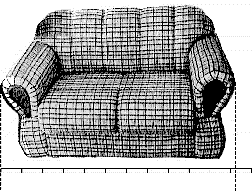
\includegraphics[width=200bp]{sofauerj99.png}
\caption{Prova de acesso UERJ 1999}
\label{\detokenize{NO103-A:fig-uerj99-sofa}}
\label{\detokenize{NO103-A:id1}}
\end{figure}

Colocando 12 vezes a régua na direção do comprimento, sobraram 15 cm da régua; por outro lado, estendendo 11 vezes, faltaram 5 cm para atingir o comprimento total. O comprimento do sofá, em centímetros, equivale a:

$\text{(A)}\, 240$

$\text{(B)}\, 235$

$\text{(C)}\, 225$

$\text{(D)}\, 220$

\item Terra Ronca, interior de Goiás, Brasil, é um lugar famoso pelas galerias  que adentram as montanhas.

\begin{figure}[H]
\centering
\capstart

\noindent\includegraphics[width=400bp]{{LA_Exerc_2}.png}
\caption{Fotos capturardas por Luiz Amorim Duarte}\label{\detokenize{NO103-A:fig-terra-ronca}}\label{\detokenize{NO103-A:id2}}\end{figure}

Durante a trilha uma pessoa observou uma rocha muito grande que, de acordo com sua disposição na trilha, havia se desprendido e caído no rio recentemente.

\begin{figure}[H]
\centering
\capstart

\noindent\includegraphics[width=250bp]{{DSC08419}.jpg}
\caption{Foto capturada por Luiz Amorim Duarte}\label{\detokenize{NO103-A:fig-rocha-caida-terra-ronca}}\label{\detokenize{NO103-A:id3}}\end{figure}

Por curiosidade, a pessoa resolveu fazer uma estimativa do peso da rocha e para isso procurou uma outra rocha menor que pudesse verificar o peso posteriormente. Por tratar-se de uma estimativa rudimentar, a pessoa considerou as rochas como paralelepípedos (caixa de faces retangulares) e estimou que a rocha selecionada para comparação cabia, aproximadamente, 8 vezes na largura, 22 vezes no comprimento e 9 vezes na altura da rocha recém caída no rio.

\begin{figure}[H]
\centering
\capstart

\noindent\includegraphics[width=300bp]{{DSC08420}.jpg}
\caption{Foto capturada por Luiz Amorim Duarte}\label{\detokenize{NO103-A:fig-coloque-aqui-o-nome}}\label{\detokenize{NO103-A:id4}}\end{figure}

Mais tarde, a pessoa pesou a rocha usada como referência, encontrando $1\text{,}3$ kg.

Nessas condições, qual o peso estimado da rocha recém caída no rio?

\item \textbf{(UERJ 2000)} Leia atentamente os quadrinhos.

\begin{figure}[H]
\centering
\capstart

\noindent\includegraphics[width=350bp]{{LA_UERJ2000_1}.png}
\caption{(O Globo, 04/09/99)}\label{\detokenize{NO103-A:fig-uerj-2000}}\label{\detokenize{NO103-A:id5}}\end{figure}

O personagem é conduzido, em linha reta, num mesmo sentido, por uma distância de 30 m e cada passo mede 50 cm. Se um dos carregadores cobrar conforme o padrão indicado, ele receberá, em reais, a quantia de:

$\text{(A)}\, 400$

$\text{(B)}\, 500$

$\text{(C)}\, 600$

$\text{(D)}\, 700$

\item \textbf{(UERJ 2001)} Os 4,5 bilhões de anos de existência da Terra podem ser reduzidos a apenas 1 ano, adotando-se a seguinte escala:

$1$ minuto = $9 \times 10^3$ anos

Desse modo, se o aparecimento dos primeiros mamíferos se deu em 16 de dezembro, os primeiros primatas surgem em 25 de dezembro.
Utilizando-se a escala, a ordem de grandeza, em séculos, entre estas duas datas é igual a:

$\text{(A)}\, 10^8$

$\text{(B)}\, 10^6$

$\text{(C)}\, 10^4$

$\text{(D)}\, 10^2$

\item Em um site de memes, encontra-se a imagem a seguir, que brinca com os prefixos do SI:

\begin{figure}[H]
\centering
\capstart

\noindent\includegraphics[width=300bp]{{LA_Exec_MEME}.jpg}
\caption{\url{https://es.memedroid.com/memes/detail/2187866}}\label{\detokenize{NO103-A:fig-umog-meme}}\label{\detokenize{NO103-A:id6}}\end{figure}

Perceba que a ideia é considerar uma unidade chamada \emph{peuta}, que é a menor das imagens. Depois as ampliações recebem os prefixos do SI: kilo, Mega, Giga e Tera, para formar a palavra \emph{TERAPEUTA}.
\begin{enumerate}
\item {} 
Considere que a menor das imagens tem 2 cm de altura; Afim de manter a relação descrita no SI para as alturas das imagens, qual deveria ser a altura da imagem cujo nome é \emph{TERAPEUTA}?

\item {} 
Como a proposta é que \emph{peuta} seja a unidade, o que seria mais correto para a imagem \emph{TERAPEUTA}?

$\Box$ Ter área igual a $10^{12}$ \emph{peutas}.

$\Box$ Ter $10^{12}$ imagens iguais a imagem \emph{peuta}.

$\Box$ Ter uma terapeuta com um cabelo $10^{12}$ mais volumoso.

\end{enumerate}



\item Foi gravado e editado um filme em alta definição com cerca de 1 hora e 30 minutos tendo como resultado final cerca de 9,5 GB.
\begin{enumerate}
\item {} 
Quantos DVDs-5 serão necessários para gravar este filme?

\item {} 
Poderíamos usar outra mídia para gravar este filme?

\end{enumerate}

\item Luiz tem várias apostilas que, em média, ocupam 2,8 MB cada uma. Ele decidiu imprimir essas apostilas. Para isso, terá que levar essas apostilas para a gráfica com que já trabalha e ela só recebe arquivos em CD.
\begin{enumerate}
\item {} 
Quantos megabytes cabem em um CD comum de uma camada?

\item {} 
Quantas apostilas o Luiz consegue colacar em média em um CD?

\end{enumerate}

\item Bruno tem uma conexão em sua casa de 20 Mbps, ou seja, 20 megabits por segundo. Ele começou a fazer o download de um filme em 4K com 27 GB. Nessas condições, quantas horas serão necessárias para a conclusão do download?

\item O dia 10 de abril de 2019 entrou para história da ciência ao ser divulgada a primeira foto de um buraco negro. As informações que envolvem o feito inédito impressionam, de acordo com a matéria \href{https://www1.folha.uol.com.br/ciencia/2019/04/conheca-katie-bouman-a-cientista-responsavel-pela-imagem-do-buraco-negro.shtml}{Conheça Katie Bouman, a cientista responsável pela imagem do buraco negro}, Katie explica que fotografar um buraco negro se compara a  “\emph{fotografar uma laranja na lua, mas com um radiotelescópio. Imaginar algo tão pequeno significa que precisaríamos de um telescópio com 10 mil quilômetros de diâmetro, o que não é prático, porque o diâmetro da Terra não chega a 13 mil quilômetros}”.

Para a conclusão da foto, 8 observatórios ao redor do mundo foram interligados para formar um grande telescópio virtual. Foram cinco dias de registros de imagens, produzindo um total de  5 petabytes de informações que, processadas, gerou a 1ª foto de um buraco negro da história:

\begin{figure}[H]
\centering
\capstart

\noindent\includegraphics[width=300bp]{{2319_blackhole_1600}.jpg}
\caption{Imagem disponível em: \url{https://solarsystem.nasa.gov/resources/2319/first-image-of-a-black-hole/}}\label{\detokenize{NO103-A:fig-umog-exec-medida-informatica-buraco-negro}}\label{\detokenize{NO103-A:id7}}\end{figure}

Para se entender a dificuldade de processar 5 petabytes de informações, faça o que se pede:
\begin{enumerate}
\item {} 
Quantos discos Blu-ray, com capacidade de 25 GB seriam necessários para armazenar os 5 PB citados no texto?

\item {} 
Pesquise o que significa o termo Mbps.

\item {} 
No endereço eletrônico \url{https://www.speedtest.net/global-index}, encontramos as campeãs de velocidade de internet móvel no mundo. No momento de elaboração deste item, a velocidade média para internet móvel, dentre os dez primeiros países, era de 64,8Mbps. Com essa velocidade, qual o tempo para transferir os 5 PB de informações?

\end{enumerate}


\label{\detokenize{NO103-A:praticando-da-secao-grandezas-compostas}}
\item Calcule o IMC de Maria, uma jovem de 21 anos,  que mede 1,82 m e pesa 60 kg.  Ela  está  fazendo uma dieta para perder peso. Verifique em que situação ela se encontra, segundo ao quadro a seguir:

\begin{table}[H]
\centering
\caption{Fonte:\href{http://portalms.saude.gov.br/component/content/article/804-imc/40509-imc-em-adultos}{Ministério da Saúde}}
\begin{tabu} to \textwidth{|l|c|}
\hline
\thead
IMC
&
Situação
\\
\hline
Abaixo de 18,5
&
Baixo peso
\\
\hline
De 18,5(inclusive) até
25(exclusive)
&
Peso ideal
\\
\hline
De 25 (inclusive) até
30(exclusive)
&
Sobrepeso
\\
\hline
De 30 em diante
&
Obesidade
\\
\hline
\end{tabu}
\end{table}

\item Se o PIB de um país aumentar $50\%$ e sua população crescer $20\%$ no mesmo período, o PIB per capita após este período aumentará ou diminuirá? Se o PIB per capita incial for $V$,  quanto valerá o PIB per capita final, que denotaremos por $V'$, em função de $V$?

\item Observe o quadro a seguir:

\begin{table}[H]
\centering
\caption{Fonte: \href{https://www.cia.gov/library/publications/the-world-factbook/rankorder/2004rank.html}{Centra Intelligence Agency (CIA)}}
\begin{tabu} to \textwidth{|l|r|r|r|}
\hline
\thead
\makecell{\centering Países} & \makecell{ PIB per capita - 2017\\ (em  ólares/ nº de\\ habitantes)} & \makecell{ População \\ aproximada (em 2017) \\ população mundial:} & \makecell{Área km$^{\text 2}$} \\
\hline
África do Sul & 13.500 & 54.841.552 & 1.219.090 \\
\hline
Brasil & 15.600 & 207.353.391 & 8.515.770 \\ 
\hline
China & 16.700 & 1.379.302.771 & 9.596.960 \\
\hline
Cuba & 12.300 & 11.147.407 & 110.860 \\ 
\hline
Estados Unidos & 59.500 & 326.625.791 & 9.833.517 \\
\hline
Grécia & 27.700 & 10.768.477 & 131.957 \\ 
\hline
Haiti & 1.800 & 10.646.714 & 27.750 \\
\hline
Finlândia & 44.300 & 5.518.371 & 338.145 \\
\hline
Rússia & 27.800 & 142.257.519 & 17.098.242 \\
\hline
Venezuela & 12.100 & 31.304.016 & 912.050 \\
\hline
\end{tabu}
\end{table}

\begin{enumerate}
\item {} 
Olhando os dados da tabela, estime qual dos países possui o maior PIB.

\item {} 
Entre os países que aparecem na  tabela, identifique o que possui maior densidade demográfica    e o de  menor densidade demográfica. Dica: Use estimativas para evitar fazer o cálculo da densidade demográfica de todos os países.

\end{enumerate}

\item O quadro a seguir apresenta a densidade absoluta, também chamada de massa específica de algumas substâncias, nas condições padrão de temperatura e pressão.

\begin{table}[H]
\centering
\begin{tabu} to \textwidth{|l|c|}
\hline
\thead
Substância
&
Densidade absoluta ou massa específica (g/cm$^{\text{3}}$)
\\
\hline
Água
&
1
\\
\hline
Água do mar
&
1,03
\\
\hline
Alumínio
&
2,7
\\
\hline
Cortiça
&
0,24
\\
\hline
Madeira
&
0,5
\\
\hline
\end{tabu}
\end{table}


Usando as informações do quadro anterior, decida o que acontecerá em cada situação a seguir. Justifique sua opinião.

\begin{table}[H]
\centering
\begin{tabu} to \textwidth{|l|c|c|}
\hline
\thead
Situação
&
Afunda ou flutua?
&
Justificativa
\\
\hline
Um barco de madeira na água do mar
&&\\
\hline
Um barco de alumínio na água do mar
&&\\
\hline
Uma rolha de cortiça em um copo d’água
&&\\
\hline
Um copo de alumínio numa bacia d’água
&&\\
\hline
Um anel de alumínio num copo dágua
&&\\
\hline
\end{tabu}
\end{table}


\item\textbf{(ENEM-2016)}  Densidade absoluta ($d$) é a razão entre a massa de um corpo e o volume por ele ocupado. Um professor propôs à sua turma que os alunos analisassem a densidade de três corpos: $d_{A}$, $d_{B}$, $d_{C}$ os alunos verificaram que o corpo $A$ possuía $1\text{,}5$ vez a massa do corpo $B$ e esse, por sua vez, tinha $\frac{3}{4}$ da massa do corpo $C$. Observaram, ainda, que o volume do corpo $A$ era o mesmo do corpo $B$ e $20\%$ maior do que o volume do corpo $C$.

Após a análise, os alunos ordenaram corretamente as densidades desses corpos da seguinte maneira
\begin{enumerate}
\item {} 
$d_{B} < d_{A} < d_{C}$

\item {} 
$d_{B} = d_{A} < d_{C}$

\item {} 
$d_{C} < d_{B} = d_{}$

\item {} 
$d_{B} < d_{C} < d_{A}$

\item {} 
$d_{C} < d_{B} < d_{A}$

\end{enumerate}
\end{enumerate}

\ifnum\aluno=1
\clearpage
\else
\notasfinais
\fi

\bibliographystyle{apalike-pt}
\bibliography{../Bibliografia/financeira_bibliografia.bib}

\nocite{*}